\documentclass[a4paper, 10pt, ]{article}

\usepackage[slovak]{babel}





\usepackage[utf8]{inputenc}
\usepackage[T1]{fontenc}

\usepackage[left=4cm,
			right=4cm,
            % left=2.5cm,
			% right=5.5cm,
			top=2.1cm,
			bottom=2.6cm,
			footskip=7.5mm,
			% twoside,
			marginparwidth=3.0cm,
			%showframe,
			]{geometry}

\usepackage{graphicx}
\usepackage[dvipsnames]{xcolor}
% https://en.wikibooks.org/wiki/LaTeX/Colors


% ------------------------------

\usepackage{lmodern}

\usepackage[tt={oldstyle=false,proportional=true,monowidth}]{cfr-lm}

% ------------------------------

\usepackage{amsmath}
\usepackage{amssymb}
\usepackage{amsthm}

\usepackage{booktabs}
\usepackage{multirow}
\usepackage{array}
\usepackage{dcolumn}


\usepackage[singlelinecheck=true]{subfig}


% ------------------------------


\def\naT{\mathsf{T}}

\hyphenpenalty=6000
\tolerance=1000




% ------------------------------


\makeatletter

	\def\@seccntformat#1{\protect\makebox[0pt][r]{\csname the#1\endcsname\hspace{4mm}}}

	\def\cleardoublepage{\clearpage\if@twoside \ifodd\c@page\else
	\hbox{}
	\vspace*{\fill}
	\begin{center}
	\phantom{}
	\end{center}
	\vspace{\fill}
	\thispagestyle{empty}
	\newpage
	\if@twocolumn\hbox{}\newpage\fi\fi\fi}

	\newcommand\figcaption{\def\@captype{figure}\caption}
	\newcommand\tabcaption{\def\@captype{table}\caption}

\makeatother


% ------------------------------




\usepackage{fancyhdr}
\fancypagestyle{plain}{%
\fancyhf{} % clear all header and footer fields
\fancyfoot[C]{\sffamily {\bfseries \thepage}\ | {\scriptsize\oznacenieCasti}}
\renewcommand{\headrulewidth}{0pt}
\renewcommand{\footrulewidth}{0pt}}
\pagestyle{plain}


% ------------------------------


\usepackage{titlesec}
\titleformat{\paragraph}[hang]{\sffamily  \bfseries}{}{0pt}{}
\titlespacing*{\paragraph}{0mm}{3mm}{1mm}
\titlespacing*{\subparagraph}{0mm}{3mm}{1mm}

\titleformat*{\section}{\sffamily\Large\bfseries}
\titleformat*{\subsection}{\sffamily\large\bfseries}
\titleformat*{\subsubsection}{\sffamily\normalsize\bfseries}






% ------------------------------

\PassOptionsToPackage{hyphens}{url}
\usepackage[pdfauthor={},
			pdftitle={},
			pdfsubject={},
			pdfkeywords={},
			% hidelinks,
			colorlinks=false,
			breaklinks,
			]{hyperref}


% ------------------------------


\graphicspath{%
{../fig_standalone/}%
{../../PY/fig/}%
{../../PY/jupynotex/fig/}%
{../../ML/fig/}%
{./fig/}%
}



% ------------------------------

\usepackage{enumitem}

\usepackage{lettrine}

% ------------------------------


\usepackage{microtype}


% ------------------------------

\usepackage[titles]{tocloft}

\setlength{\cftsecindent}{-12mm}
\setlength{\cftsecnumwidth}{12mm}
\renewcommand{\cftsecpresnum}{\hfill}
\renewcommand{\cftsecaftersnum}{\hspace{4mm}}

\setlength{\cftsubsecindent}{-12mm}
\setlength{\cftsubsecnumwidth}{16mm} % 12 + 4
\renewcommand{\cftsubsecpresnum}{\hfill}
\renewcommand{\cftsubsecaftersnum}{\hspace{8mm}} % 4 + 4 mm

\setlength{\cftsubsubsecindent}{-12mm}
\setlength{\cftsubsubsecnumwidth}{20mm} % 12 + 4 + 4
\renewcommand{\cftsubsubsecpresnum}{\hfill}
\renewcommand{\cftsubsubsecaftersnum}{\hspace{12mm}} % 4 + 4 + 4 mm

\renewcommand{\cftsecpagefont}{\lstyle \bfseries}
\renewcommand{\cftsubsecpagefont}{\lstyle}
\renewcommand{\cftsubsubsecpagefont}{\lstyle}



\setlength{\cftparaindent}{-16mm}
\setlength{\cftparanumwidth}{28mm} % 16 + 4 + 4 + 4
\renewcommand{\cftparapresnum}{\hfill}
\renewcommand{\cftparaaftersnum}{\hspace{16mm}} % 4 + 4 + 4 + 4 mm








% ------------------------------

\usepackage{listings}



\renewcommand{\lstlistingname}{Výpis kódu}
\renewcommand{\lstlistlistingname}{Výpisy kódu}




%New colors defined below
\definecolor{codegreen}{rgb}{0,0.6,0}
\definecolor{codegray}{rgb}{0.5,0.5,0.5}
\definecolor{codepurple}{rgb}{0.58,0,0.82}
\definecolor{backcolour}{rgb}{0.95,0.95,0.95}

%Code listing style named "mystyle"
\lstdefinestyle{mystyle}{
  backgroundcolor=\color{backcolour},
  commentstyle=\fontfamily{lmtt}\fontsize{8.5pt}{8.75pt}\selectfont\color{codegreen},
  keywordstyle=\fontfamily{lmtt}\fontsize{8.5pt}{8.75pt}\selectfont\bfseries\color{Blue},
  stringstyle=\fontfamily{lmtt}\fontsize{8.5pt}{8.75pt}\selectfont\color{codepurple},
  basicstyle=\fontfamily{lmtt}\fontsize{8.5pt}{8.75pt}\selectfont,
  breakatwhitespace=false,
  breaklines=true,
  captionpos=t,
  keepspaces=true,
  numbers=left,
  numbersep=4mm,
  numberstyle=\fontfamily{lmtt}\fontsize{8.5pt}{8.75pt}\selectfont\color{lightgray},
  showspaces=false,
  showstringspaces=false,
  showtabs=false,
  tabsize=2,
  % xleftmargin=10pt,
  framesep=10pt,
  language=Python,
  escapechar=|,
}


\lstset{
    inputencoding=utf8,
    extendedchars=true,
    literate=%
    {á}{{\'a}}1
    {č}{{\v{c}}}1
    {ď}{{\v{d}}}1
    {é}{{\'e}}1
    {ě}{{\v{e}}}1
    {í}{{\'i}}1
    {ň}{{\v{n}}}1
    {ó}{{\'o}}1
    {ř}{{\v{r}}}1
    {š}{{\v{s}}}1
    {ť}{{\v{t}}}1
    {ú}{{\'u}}1
    {ů}{{\r{u}}}1
    {ý}{{\'y}}1
    {ž}{{\v{z}}}1
    {Á}{{\'A}}1
    {Č}{{\v{C}}}1
    {Ď}{{\v{D}}}1
    {É}{{\'E}}1
    {Ě}{{\v{E}}}1
    {Í}{{\'I}}1
    {Ň}{{\v{N}}}1
    {Ó}{{\'O}}1
    {Ř}{{\v{R}}}1
    {Š}{{\v{S}}}1
    {Ť}{{\v{T}}}1
    {Ú}{{\'U}}1
    {Ů}{{\r{U}}}1
    {Ý}{{\'Y}}1
    {Ž}{{\v{Z}}}1
    {ô}{{\^{o}}}1
}


% ------------------------------


\usepackage{caption}

\DeclareCaptionFormat{odsadene}{\protect\makebox[0pt][r]{#1#2\hspace{4mm}}#3\par}
\DeclareCaptionLabelSeparator{lendvojbodka}{:}
% \DeclareCaptionFont{lightgray}{\color{lightgray}}
\DeclareCaptionFont{lightgray}{\fontfamily{lmtt}\fontsize{8.5pt}{8.75pt}\selectfont\color{lightgray}}

\captionsetup[lstlisting]{format=odsadene, labelsep=lendvojbodka, justification=raggedright, singlelinecheck=false, labelfont={sf, lightgray},}


% ------------------------------





% ------------------------------

\usepackage[backend=biber,
            style=numeric,
            sorting=none,
            ]{biblatex}
\DeclareSourcemap{
    \maps[datatype=bibtex]{
        \map{
        \step[fieldset=note, null]
        }
        \map{
        \step[fieldset=file, null]
        }        
        % \map{
        % \step[fieldset=url, null]        
        % }
        \map{
        \step[fieldset=eprint, null]
        }
    }
}


\addbibresource{E:/_CurrentContent/01_work_repo/bibLaTeXDB/bibLaTeXDB.bib} % nonpublic data





\def\oznacenieCasti{AR05 - LS2025}





\begin{document}

\lstset{%
style=mystyle,
rangebeginprefix=\#\#\#\ cellB\ ,%
rangebeginsuffix=\ \#\#\#,%
rangeendprefix=\#\#\#\ cellE\ ,%
rangeendsuffix=\ \#\#\#,%
includerangemarker=false,
}




\fontsize{12pt}{22pt}\selectfont

\centerline{\textsf{Adaptívne riadenie} \hfill \textsf{\oznacenieCasti}}

\fontsize{18pt}{22pt}\selectfont








\begin{flushleft}
    \textbf{\textsf{MRAC stavový}}
\end{flushleft}







\normalsize

\bigskip

{\hypersetup{hidelinks}

\tableofcontents

}

\bigskip

\vspace{18pt}






\noindent
\lettrine[lines=3, nindent=0pt]{V}{} tejto časti využijeme pri návrhu mechanizmu adaptácie Lyapunovovu teóriu stability. Najprv je však potrebné opísať neadaptívny riadiaci systém, ktorý neskôr doplníme zákonom adaptácie.












\section{Stavový regulátor}
\label{Stavový regulátor ($n=2$)}


Uvažujme riadený systém, ktorý je zadaný nasledujúcou sústavou rovníc
\begin{subequations} \label{system2radu}
\begin{align}
    \dot x_1 &= x_2  &  x_1(0)&=0 \\
    \dot x_2 &= -a_1 x_2 - a_0 x_1 + b_0 u &  x_2(0)&=0 \\
    y &= x_1
\end{align}
\end{subequations}
kde $y(t)$ je výstupná veličina riadeného systému, $u(t)$ je vstupná veličina (akčný zásah), $x_1(t)$, $x_2(t)$ sú stavové veličiny systému a $a_0$, $a_1$, $b_0$ sú reálne konštanty -- parametre riadeného systému. Rovnice \eqref{system2radu} je možné zapísať v maticovom tvare:
\begin{subequations} \label{maticformasystemu2r}
    \begin{align}
        \begin{bmatrix} \dot x_1  \\ \dot x_2 \end{bmatrix}
         &=
         \begin{bmatrix} 0 & 1 \\ -a_0 & -a_1 \end{bmatrix}
         \begin{bmatrix} x_1 \\ x_2 \end{bmatrix}
         +
         \begin{bmatrix} 0 \\ b_0 \end{bmatrix}
         u \\
         y &= \begin{bmatrix} 1 & 0 \end{bmatrix}
         \begin{bmatrix} x_1 \\ x_2 \end{bmatrix}
    \end{align}
\end{subequations}
Tvar \eqref{maticformasystemu2r} budeme nazývať \emph{opis v stavovom priestore} (alebo skrátene: stavový opis). Vstupno výstupný opis systému \eqref{system2radu} v tvare prenosovej funkcie je
\begin{equation} \label{k01:eq:02}
    \frac{y(s)}{u(s)}
    =
    \begin{bmatrix} 1 & 0 \end{bmatrix}
     \left(
         s \begin{bmatrix} 1 & 0 \\ 0 & 1 \end{bmatrix}
         -
         \begin{bmatrix} 0 & 1 \\ -a_0 & -a_1 \end{bmatrix}
     \right)^{-1}
     \begin{bmatrix} 0 \\ b_0 \end{bmatrix}
     =
     \frac{b_0}{s^2 + a_1 s + a_0}
\end{equation}

Navrhnime \emph{stavový regulátor}, ktorý zabezpečí, že stavový opis uzavretého regulačného obvodu sa zhoduje so stavovým opisom referenčného modelu. Inými slovami, nech priebeh stavových veličín URO, ktorými sú stavové veličiny riadeného systému, je zhodný s~priebehom stavových veličín referenčného modelu. Uvažujme teda referenčný model s~rovnakým počtom veličín (stavových, výstupných, vstupných) ako riadený systém v~tvare
\begin{subequations}
    \begin{align}
        \begin{bmatrix} \dot x_{1m} \\ \dot x_{2m} \end{bmatrix}
         &=
         \begin{bmatrix} 0 & 1 \\ -a_{0m} & -a_{1m} \end{bmatrix}
         \begin{bmatrix} x_{1m} \\ x_{2m} \end{bmatrix}
         +
         \begin{bmatrix} 0 \\ b_{0m} \end{bmatrix}
         r
         \label{stavovyOpisRM2R} \\
         y_m
         &=
         \begin{bmatrix} 1  & 0 \end{bmatrix}
         \begin{bmatrix} x_{1m} \\ x_{2m} \end{bmatrix}
    \end{align}
\end{subequations}
kde $y_m(t)$ je vystupná veličina referenčného modelu, $r(t)$ je referenčný signál (podobne ako žiadaná hodnota), $x_{1m}(t)$, $x_{2m}(t)$ sú stavové veličiny referenčného modelu a $a_{0m}$, $a_{1m}$, $b_{0m}$ sú reálne konštanty -- parametre referenčného modelu.








Stavový regulátor (stavový zákon riadenia) v tvare
\begin{equation} \label{stavZakRiad2r}
    u =
    \begin{bmatrix} k_1 & k_2 \end{bmatrix}
    \begin{bmatrix} x_1 \\ x_2 \end{bmatrix}
    + l \, r
\end{equation}
kde $k_1$, $k_2$, $l$ sú reálne konštanty -- parametre regulátora (zosilnenia regulátora) spĺňa danú úlohu ako plynie z nasledujúceho.



Dosadením zákona riadenia \eqref{stavZakRiad2r} do stavového opisu riadeného systému \eqref{maticformasystemu2r} sa získa stavový opis uzavretého regulačného obvodu v tvare
\begin{subequations} \label{stavopisURO2r}
    \begin{align}
        \begin{bmatrix} \dot x_1  \\ \dot x_2 \end{bmatrix}
        & =
        \begin{bmatrix} 0 & 1 \\ -a_0 & -a_1 \end{bmatrix}
        \begin{bmatrix} x_1 \\ x_2 \end{bmatrix}
        +
        \begin{bmatrix} 0 \\ b_0 \end{bmatrix}
        \left(
            \begin{bmatrix} k_1 & k_2 \end{bmatrix}
            \begin{bmatrix} x_1 \\ x_2 \end{bmatrix}
            + l \, r
        \right) \\
        y &=
         \begin{bmatrix} 1 & 0 \end{bmatrix}
         \begin{bmatrix} x_1 \\ x_2 \end{bmatrix}
    \end{align}
\end{subequations}
a po úpravách (rovnicu výstupnej veličiny neuvádzame, pretože sa nemení)
\begin{align}
    \begin{bmatrix} \dot x_1 \\ \dot x_2 \end{bmatrix}
    &=
    \left(
        \begin{bmatrix} 0 & 1 \\ -a_0 & -a_1 \end{bmatrix}
         +
         \begin{bmatrix} 0 \\ b_0 \end{bmatrix}
         \begin{bmatrix} k_1 & k_2 \end{bmatrix}
    \right)
    \begin{bmatrix} x_1  \\ x_2 \end{bmatrix}
    +
    \begin{bmatrix} 0  \\ b_0 \end{bmatrix}
    l \, r
    \\
    \begin{bmatrix} \dot x_1 \\ \dot x_2 \end{bmatrix}
    &=
    \left(
        \begin{bmatrix} 0 & 1 \\ -a_0 & -a_1 \end{bmatrix}
         +
         \begin{bmatrix} 0 & 0 \\ b_0 k_1 & b_0 k_2 \end{bmatrix}
    \right)
    \begin{bmatrix} x_1  \\ x_2 \end{bmatrix}
    +
    \begin{bmatrix} 0  \\ b_0 l \end{bmatrix}
    r
    \\
    \begin{bmatrix} \dot x_1 \\ \dot x_2 \end{bmatrix}
    &=
    \begin{bmatrix} 0 & 1 \\ -a_0 + b_0 k_1 & -a_1 + b_0 k_2 \end{bmatrix}
    \begin{bmatrix} x_1  \\ x_2 \end{bmatrix}
    +
    \begin{bmatrix} 0  \\ b_0 l \end{bmatrix}
    r
    \label{RAWstavopisURO2r}
\end{align}
Ak žiadame $x_1 = x_{1m}$ a $x_2 = x_{2m}$ potom z porovnania \eqref{RAWstavopisURO2r} a \eqref{stavovyOpisRM2R} plynie
\begin{subequations}
    \begin{align}
        -a_0 + b_0 k_1 &=  -a_{0m}\\
        -a_1 + b_0 k_2 &=  -a_{1m}\\
        b_0 l &= b_{0m}
    \end{align}
\end{subequations}
odkiaľ
\begin{subequations}
    \begin{align}
        k_1 &= \frac{ -a_{0m} + a_0}{b_0}\\
        k_2 &= \frac{ -a_{1m} + a_1}{b_0}\\
        l &= \frac{b_{0m}}{b_0}
    \end{align}
\end{subequations}
sú parametre regulátora \eqref{stavZakRiad2r}, ktoré spĺňajú cieľ.

Vyššie uvedené sa zvyčajne zapisuje v kratšom tvare nasledovne. Uvažujeme riadený systém v tvare
\begin{subequations} \label{sustavavSS2r}
    \begin{align}
         \dot x &= A x + b u \\
         y &= c^\naT x
    \end{align}
\end{subequations}
pričom ak v tomto tvare zapisujeme sústavu rovníc \eqref{system2radu} potom
\begin{align*}
    x &= \begin{bmatrix} x_1 \\ x_2 \end{bmatrix}
    &
    A &= \begin{bmatrix} 0 & 1 \\ -a_0 & -a_1 \end{bmatrix}
    &
    b &= \begin{bmatrix} 0 \\ b_0 \end{bmatrix}
    &
    c &= \begin{bmatrix} 1 \\ 0 \end{bmatrix}
\end{align*}

Pre prepočet opisu v stavovom priestore \eqref{sustavavSS2r} na vstupno-výstupný opis v tvare prenosovej funkcie platí vzťah
\begin{equation}
    \frac{y(s)}{u(s)} = c^\naT \left( s I - A \right)^{-1} b
\end{equation}

Systém rovníc \eqref{sustavavSS2r} možno vyjadriť blokovou schémou na Obr.~\ref{orsvsp:fig:01}.







\begin{figure}[t]
    \centering
    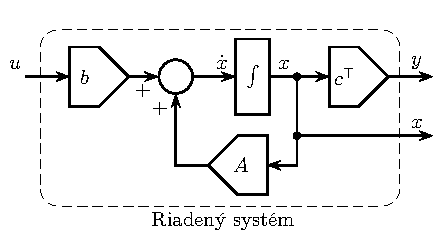
\includegraphics{Obr_ssSYSblokSch_standalone.pdf}

    % \vspace{5mm}

    \caption{Bloková schéma systému \eqref{sustavavSS2r}}
    \label{orsvsp:fig:01}

    % \vspace{5mm}

\end{figure}










Podobne referenčný model
\begin{subequations}
    \begin{align}
         \dot x_m &= A_m x_m + b_m r \\
         y_m &= c_m^\naT x_m
    \end{align}
\end{subequations}
kde v predchádzajúcom príklade
\begin{align*}
    x_m &= \begin{bmatrix} x_{1m} \\ x_{2m} \end{bmatrix}
    &
    A_m &= \begin{bmatrix} 0 & 1 \\ -a_{0m} & -a_{1m} \end{bmatrix}
    &
    b_m &= \begin{bmatrix} 0 \\ b_{0m} \end{bmatrix}
    &
    c_m &= \begin{bmatrix} 1 \\ 0 \end{bmatrix}
\end{align*}

Zákon riadenia stavového regulátora má vo všeobecnosti tvar
\begin{equation}
    u = k^\naT x + l r
\end{equation}
kde $k^\naT$ je vektor parametrov (zosilnení) spätnoväzbového člena a v predchádzajúcom príklade $k^\naT = \begin{bmatrix} k_1 & k_2 \end{bmatrix}$ a $l$ zosilnenie dopredného člena. V niektorých prípadoch je výhodné zapísať zákon riadenia v tvare
\begin{equation} \label{vseobecnyZapisU2r}
    u = \Theta^\naT \omega
\end{equation}
kde $\Theta$ je vektor parametrov zákona riadenia a $\omega$ je tzv. signálny vektor (vektor obsahujúci signály). V predchádzajúcom príklade je $\Theta^\naT = \begin{bmatrix} k^\naT & l \end{bmatrix}$ a $\omega^\naT = \begin{bmatrix} x^\naT & r  \end{bmatrix}$. Do tvaru \eqref{vseobecnyZapisU2r} je možné zapísať v podstate akýkoľvek zákon riadenia (regulátor).

Uzavretý regulačný obvod so stavovým regulátorom:
\begin{subequations}
    \begin{align}
         \dot x &= A x + b \left( k^\naT x + l r \right)\\
         y &= c^\naT x
    \end{align}
\end{subequations}
Po úprave
\begin{align}
    \dot x = \left( A + b k^\naT \right) x + b l r
\end{align}
Parametre stavového regulátora sa získajú riešením sústavy algebraických rovníc v~tvare
\begin{subequations} \label{podmienkyZhody2r}
    \begin{align}
        A + b k^\naT & = A_m \\
        b l &= b_m
    \end{align}
\end{subequations}
Tieto rovnice sa v adaptívnom riadení nazývajú \emph{podmienky zhody}. Ich splnenie znamená, že URO sa správa rovnako ako referenčný model, a to je cieľom riadenia.

Ďalšou úpravou, v ktorej využijeme funkciu \verb+pinv+(), v~rovnakom význame ako sa používa v \textsc{Matlab}-e, možno priamo vyjadriť parametre stavového regulátora v tvare
\begin{equation*}
    k^\naT = \verb|pinv|(b) \left( A_m - A \right) \qquad l = \verb|pinv|(b) b_m
\end{equation*}








\section{MRAC so stavovou štruktúrou riadenia}


V tejto časti odvodíme adaptívny algoritmus riadenia, ktorý sa zaraďuje do triedy Priame adaptívne riadenie. Pripomeňme Priame adaptívne riadenie:

\noindent
Model riadeného systému je parametrizovaný pomocou ideálnych parametrov zákona riadenia. To znamená, že rovnica modelu riadeného systému je vyjadrená tak, že obsahuje ideálne parametre zákona riadenia. Pretože najmä tieto parametre sú neznáme, sú priebežne identifikované -- adaptované. Výstupom priebežnej identifikácie (zákona adaptácie) sú teda priamo parametre zákona riadenia. Nie je potrebný medzivýpočet ako v prípade nepriameho adaptívneho riadenia.

Pri odvodení zákona riadenia sa v tejto časti bude využívať Ljapunovova priama metóda na rozdiel od využitia gradientného prístupu (aký sa využíva pri MIT pravidle - ktoré sme my nazvali ako MRAC gradientný).


\subsection{Frobeniov kanonický tvar matice $A$}

V tomto prípade uvažujeme zákon riadenia v tvare \emph{stavového regulátora}. To znamená, že predpokladáme riadený systém, ktorého model má štruktúru vhodnú pre použitie práve stavového regulátora. Presnejšie, ak v SISO systéme, napr. \eqref{sustavavSS2r}, opísanom v stavovom priestore má matica $A$ istú kanonickú formu --- nazývanú \emph{Frobeniov kanonický tvar matice}, tak existuje riešenie podmienok zhody, akými sú \eqref{podmienkyZhody2r}. Ak matica $A$ nemá Frobeniov kanonický tvar potom nie je možné splniť podmienky zhody, a teda nie je možné navrhnúť -- vypočítať parametre stavového regulátora. Frobeniov kanonický tvar matice vo všeobecnosti je:
\begin{equation}
    A
    =
    \begin{bmatrix}
      0      & 1      & 0      & \cdots & 0      & 0      \\
       0      & 0      & 1      & \ddots & 0      & 0      \\
    \vdots & \vdots & \ddots & \ddots & \ddots & \vdots \\
    0      & 0      & 0      & \ddots & 1      & 0      \\
    0      & 0      & 0      & \cdots & 0      & 1      \\
       -a_0   & -a_1   & -a_2   & \cdots &-a_{n-2}&-a_{n-1}
    \end{bmatrix}
\end{equation}


Ak poznáme hodnoty parametrov matíc $A$, $b$, $c$, potom je možné prepočítať ľubovoľný tvar matice $A$ do Frobeniovho kanonického tvaru.

Avšak, v adaptívnom riadení sa predpokladá, že parametre systému a teda aj matice $A$ sú neznáme. Preto nie je možné uskutočniť prepočet do Frobeniovho kanonického tvaru -- nie je možné nájsť transformačnú maticu. Z toho vyplýva, že MRAC so stavovou štruktúrou riadenia možno použiť napríklad vtedy, keď prirodzeným tvarom modelu riadeného systému je taký, že $A$~má Frobeniov kanonický tvar. Zároveň, samozrejme, stavový vektor musí byť merateľný.



\subsection{Model riadeného systému a referenčný model}

Uvažujme riadený systém, ktorého model má tvar
\begin{subequations} \label{sustavavSS2r_2}
    \begin{align}
        \dot x &= A x + b u \\
        y &= c^\naT x
    \end{align}
\end{subequations}
kde
\begin{align*}
    A &= \begin{bmatrix} 0 & 1 \\ -a_0 & -a_1 \end{bmatrix}
    &
    b &= \begin{bmatrix} 0 \\ b_0 \end{bmatrix}
    &
    c &= \begin{bmatrix} 1 \\ 0 \end{bmatrix}
\end{align*}
ďalej, $y(t)$ je výstupná veličina riadeného systémy, $u(t)$ je vstupná veličina, $x$ je vektor stavových veličín a $a_0$, $a_1$, $b_0$ sú \emph{neznáme} parametre riadeného systému, ale znamienko parametra $b_0$ je známe.


Cieľom riadenia je zvoliť vhodný algoritmus riadenia, taký že všetky signály uzavretej regulačnej slučky sú ohraničené a stavový vektor $x$ sleduje stavový vektor referenčného modelu $x_m$ daného v tvare
\begin{subequations}
    \begin{align}
        \dot x_m &= A_m x_m + b_m r \\
        y_m &= c_m^\naT x_m
        \end{align}
\end{subequations}
kde
\begin{align*}
    A_m &= \begin{bmatrix} 0 & 1 \\ -a_{0m} & -a_{1m} \end{bmatrix}
    &
    b_m &= \begin{bmatrix} 0 \\ b_{0m} \end{bmatrix}
    &
    c_m &= \begin{bmatrix} 1 \\ 0 \end{bmatrix}
\end{align*}
kde $y_m(t)$ je vystupná veličina referenčného modelu a $a_{0m}$, $a_{1m}$, $b_{0m}$ sú reálne konštanty -- parametre referenčného modelu, ktoré závisia od požiadaviek na správanie sa URO. Referenčný signál $r(t)$ je ohraničený, po častiach spojitý a predpokladá sa, že je zvolený tak (spolu s $a_{0m}$, $a_{1m}$, $b_{0m}$), že priebeh $x_m$ reprezentuje želanú reakciu riadeného systému.





\subsection{Zákon riadenia}

Ako je známe z časti \ref{Stavový regulátor ($n=2$)}, zákon riadenia v tvare
\begin{equation} \label{idealZakRiadenia2r}
    u = {k^\star}^\naT x + l^\star r
\end{equation}
zabezpečí, že priebeh stavových veličín URO, ktorými sú stavové veličiny riadeného systému, je zhodný s priebehom stavových veličín referenčného modelu ak sú parametre vypočítané z rovníc --- z podmienok zhody
\begin{subequations} \label{podmienkyZhody2r02}
    \begin{align}
        A + b {k^\star}^\naT & = A_m \\
        b l^\star &= b_m
    \end{align}
\end{subequations}

Pretože matice $A$ a $b$ obsahujú prvky s neznámou hodnotou, tak zákon riadenia \eqref{idealZakRiadenia2r} nemôže byť použitý, pretože nie je možné určiť jeho parametre (zosilnenia). Namiesto \eqref{idealZakRiadenia2r} použijeme zákon riadenia
\begin{equation} \label{estZakRiadenia2r}
    u = k^\naT(t) x + l(t) r
\end{equation}
kde $k(t)$, $l(t)$ sú odhadmi ideálnych parametrov $k^\star$, $l^\star$~v~každom čase $t$. Je potrebné nájsť \emph{Zákon adaptácie}, ktorý bude priebežne generovať hodnoty $k(t)$, $l(t)$ tak aby cieľ riadenia bol splnený.










\subsection{Zákon adaptácie}


Prvým krokom pri odvodení zákona adaptácie je parametrizácia riadeného systému pomocou ideálnych parametrov zákona riadenia. Jednoduchým pripočítaním a~odpočítaním ideálneho vstupného výrazu $+b{k^\star}^\naT x+bl^\star r$, ktorý vyplýva z ideálneho zákona riadenia \eqref{idealZakRiadenia2r} získame

\begin{align}
     \dot x &= A x + b {k^\star}^\naT x + b l^\star r - b {k^\star}^\naT x - b l^\star r + b  u
\end{align}
Pretože $A + b {k^\star}^\naT = A_m$ máme
\begin{align}
    \dot x &= A_m x + b l^\star r + b \left( u - {k^\star}^\naT x - l^\star r \right)
\end{align}
Definujme tzv. \emph{stavovú adaptačnú odchýlku}
\begin{equation}
    e = x - x_m
\end{equation}
potom
\begin{subequations}
    \begin{align}
        \dot x - \dot x_m & = A_m \left( x - x_m \right) + b l^\star r - b l^\star r + b \left( u - {k^\star}^\naT x - l^\star r \right) \\
        \dot{e} &= A_m e + b \left( u - {k^\star}^\naT x - l^\star r \right)
    \end{align}
\end{subequations}
a pri využití všeobecného zápisu zákona riadenia v tvare \eqref{vseobecnyZapisU2r}, kde zavedieme  ${\Theta^\star}^\naT = \begin{bmatrix} {k^\star}^\naT & l^\star \end{bmatrix}$ a $\omega^\naT = \begin{bmatrix} x^\naT & r  \end{bmatrix}$
\begin{equation} \label{dynStavAdaptOdch}
    \dot{e} = A_m e + b \left( u -
        {\Theta^\star}^\naT
        \omega
    \right)
\end{equation}
Rovnica \eqref{dynStavAdaptOdch} teraz predstavuje model riadeného systému parametrizovaný pomocou ideálnych parametrov zákona riadenia, od ktorého sú zavedením stavovej adaptačnej odchýlky odčítané známe zložky signálu stavových signálov, ktoré vznikli pripočítaním ideálnych vstupných výrazov (tieto zložky sú známe a~hlavne ohraničené a~teda stabilné). Neznámymi parametrami rovnice \eqref{dynStavAdaptOdch} sú vektor ${\Theta^\star}$ ale aj vektor $b$. Hodnoty týchto neznámych vektorov možno získať ich priebežnou identifikáciou.

Rovnica \eqref{dynStavAdaptOdch} predstavuje skutočný neznámy systém. Zostavíme model rovnice \eqref{dynStavAdaptOdch} s~rovnakou štruktúrou ako rovnica \eqref{dynStavAdaptOdch}, pričom skutočné signály a~parametre sú nahradené ich odhadmi
\begin{equation} \label{dynStavAdaptOdchOdhad}
    \dot{\hat e} = A_m \hat e + \hat b \left( u - \Theta^\naT(t) \omega \right)
\end{equation}
Vstupnými signálmi rovnice \eqref{dynStavAdaptOdchOdhad} sú $\omega$ a $u$. Tieto sú rovnaké aké vstupujú do skutočnej (modelovanej) rovnice \eqref{dynStavAdaptOdch}. Odhadmi neznámich parametrov sú vektor $\hat{b}$ a už vyššie nepriamo zavedený vektor $\Theta(t)$, kde zdôrazňujeme, že ide o funkciu času, pretože sa odhaduje v každom čase $t$. Je zrejmé, že cieľom identifikácie, je nájsť (identifikovať) také parametre $\hat{b}$ a ${\Theta}(t)$, pri ktorých sa bude odhad adaptačnej odchýlky $\hat{e}$ zhodovať so \uv{skutočnou} adaptačnou odchýlkou $e$. O tom či sa zhodujú hovorí \emph{chyba odhadu} $\varepsilon = e - \hat e$.

Avšak, vstup $u$ je daný zákonom riadenia \eqref{estZakRiadenia2r}, čo možno zapísať v tvare $u= \Theta^\naT(t) \omega$. Súčasne začiatočný stav odhadu $\hat e$ je prirodzene zvolený ako nulový $\hat e(0)=0$. To znamená (dosadením za $u$ do \eqref{dynStavAdaptOdchOdhad}), že $\hat e = 0; \forall t$ a preto $\varepsilon = e$. Preto pre priebežnú identifikáciu nie je potrebné generovať signál $\hat e$, namiesto neho možno použiť priamo adaptačnú odchýlku $e$. Navyše, pretože nie je potrebný $\hat e$ tak nie je potrebný ani odhad vektora $\hat b$.

Dosadením $u= \Theta^\naT(t) \omega$ do \eqref{dynStavAdaptOdchOdhad} máme
\begin{equation} \label{dynStavAdaptOdchDosad}
    \dot e = A_m e + b \left( \Theta^\naT(t) \omega - {\Theta^\star}^\naT \omega \right)
\end{equation}
V tomto bode zavedieme chybu nastavenia parametrov zákona riadenia $\theta$
\begin{equation}
    \theta = \Theta(t) - \Theta^\star
\end{equation}
potom
\begin{equation} \label{dynStavAdaptOdchChNPZR}
    \dot e = A_m e + b \left( \theta^\naT \omega \right)
\end{equation}

Zostavenie diferenciálnej rovnice \eqref{dynStavAdaptOdchChNPZR}, ktorá dáva do vzťahu chybu odhadu (identifikácie), ktorou je jednoducho adaptačná odchýlka $e$, a chybu nastavenia parametrov zákona riadenia $\theta$, je významným krokom pri odvodení zákona adaptácie pre priebežné adaptovanie prvkov vektora $\Theta(t)$.

Predpokladáme, že štruktúra zákona adaptácie je daná diferenciálnou rovnicou, všeobecne zapísanou v~tvare
\begin{equation} \label{vseobZakAdapt2r}
    \dot \theta = f \left( e, \omega \right)
\end{equation}
kde funkcia $f$ má byť určená (je predmetom návrhu). Zákon adaptácie určíme tak, aby systém tvorený diferenciálnymi rovnicami \eqref{dynStavAdaptOdchChNPZR} a \eqref{vseobZakAdapt2r} mal stabilný rovnovážny bod v $e = 0$ a $\theta = 0$, teda v začiatku spoločného priestoru vektora adaptačnej odchýlky $e$~a~chyby parametrov $\theta$.

Zvoľme kandidáta na Lyapunovovu funkciu v tvare
\begin{equation} \label{KandLjapFcn2r}
    V = e^\naT P e + \left| b_0 \right| \left( \theta^\naT \Gamma^{-1} \theta \right)
\end{equation}
kde $\Gamma^{-1} = \left( \Gamma^{-1} \right)^\naT > 0$ je ľubovolná, \emph{diagonálna}, kladne definitná matica zodpovedajúceho rozmeru a $P = P^\naT > 0$ spĺňa Lyapunovovu rovnicu
\begin{equation}
    A_m^\naT P + P A_m = - Q
\end{equation}
kde $A_m$ je matica stabilného systému (referenčného modelu) a $Q = Q^\naT > 0$ je ľubovolná symetrická kladne definitná matica rovnakého rozmeru ako $A_m$. Zápisom $\left| b_0 \right|$ značíme absolútnu hodnotu parametra $b_0$.












Každý z členov pravej strany rovnice \eqref{KandLjapFcn2r} je tzv. \emph{kvadratická forma}, čo znamená, že je to maticovo zapísaný polynóm. Napríklad v tomto prípade
\begin{align} \label{prikladP3}
    e^\naT P e
    &=
    \begin{bmatrix} e_1 & e_2 \end{bmatrix}
    \begin{bmatrix} p_1 & 0 \\ 0 & p_2 \end{bmatrix}
    \begin{bmatrix} e_1 \\ e_2 \end{bmatrix}
    =
    p_1 e_1^2 + p_2 e_2^2
\end{align}
kde sme pre jednoduchosť predpokladali, že $P$ je diagonálna (Rovnako sa však dá postupovať aj pri plnej matici pričom sa ukáže to isté). Príklad \eqref{prikladP3} predstavuje polynóm, kde vstupnými premennými sú $e_1$, $e_2$ a koeficientami polynómu sú $p_1$ a $p_2$. Je zrejmé, že \uv{výstupom} polynómu \eqref{prikladP3} je skalárna hodnota. $e_1$~a~$e_2$ sú funkciou času. Časová derivácia výrazu \eqref{prikladP3} je
\begin{align} \label{derprikladP3}
    \frac{\text{d} \left( p_1 e_1^2(t) + p_2 e_2^2(t) \right)}{\text{d}t} = 2 p_1 e_1(t) \dot{e}_1(t) + 2 p_2 e_2(t) \dot{e}_2(t)
\end{align}
Výraz \eqref{derprikladP3} je evidentne možné zapísať v rôznych (maticových) tvaroch
\begin{align} \label{rozneTvaryDerP03}
    2 e^\naT P \dot{e} = 2 \dot{e}^\naT P e = \dot{e}^\naT P e + e^\naT P \dot{e}
\end{align}
Podobne možno ukázať vlastnosti všetkých členov (kvadratických foriem) rovnice \eqref{KandLjapFcn2r}.


Časová derivácia $\dot{V}$ pozdĺž trajektórie systému \eqref{dynStavAdaptOdchChNPZR}, \eqref{vseobZakAdapt2r} je
\begin{equation} \label{derKandLjapFcn2r}
    \dot{V} = \dot{e}^\naT P e + e^\naT P \dot{e} + \left| b_0 \right| \left( \dot \theta^\naT \Gamma^{-1} \theta + \theta^\naT \Gamma^{-1} \dot \theta \right)
\end{equation}

Funkcia $V$ a aj jej derivácia $\dot{V}$ sú skalárne funkcie, myslíme tým, že ich závisle premenná („výstupná hodnota“) je skalár, pričom nezávisle premenná („vstupná/é hodnota/y“) môže byť aj vektor.


Pokračujme v úprave derivácie $\dot{V}$
\begin{align} \label{derKandLjapFcnP302}
    \dot{V} = \dot{e}^\naT P e + e^\naT P \dot{e} + \left| b_0 \right| \left( 2 \theta^\naT \Gamma^{-1} \dot \theta \right)
\end{align}
Dosadením za $\dot{e}$ \eqref{dynStavAdaptOdchChNPZR} a dosadením $\dot{e}^\naT = e^\naT A_m^\naT + \omega^\naT \theta b^\naT$ do \eqref{derKandLjapFcnP302}
\begin{align}	 \label{derKandLjapFcnP303}
    \dot{V} &= \left( e^\naT A_m^\naT + \omega^\naT \theta b^\naT \right) P e + e^\naT P \left( A_m e + b \theta^\naT \omega \right) + \left| b_0 \right| \left( 2 \theta^\naT \Gamma^{-1} \dot \theta \right) \\
    \dot{V} &= e^\naT A_m^\naT P e + \omega^\naT \theta b^\naT P e + e^\naT P A_m e + e^\naT P b \theta^\naT \omega 	+ \left| b_0 \right| \left( 2 \theta^\naT \Gamma^{-1} \dot \theta \right) \\
    \dot{V} &= e^\naT \left( A_m^\naT P + P A_m \right) e + \omega^\naT \theta b^\naT P e + e^\naT P b \theta^\naT \omega 	+ \left| b_0 \right| \left( 2 \theta^\naT \Gamma^{-1} \dot \theta \right)
\end{align}
Platí (podobne ako \eqref{rozneTvaryDerP03}) $\omega^\naT \theta b^\naT P e + e^\naT P b \theta^\naT \omega = 2 e^\naT P b  \theta^\naT \omega$, preto
\begin{align}	 \label{derKandLjapFcnP304}
    \dot{V} &= e^\naT \left( - Q \right) e + 2 e^\naT P b \theta^\naT \omega + \left| b_0 \right| \left( 2 \theta^\naT \Gamma^{-1} \dot \theta \right)
\end{align}
Prvý člen v~derivácii $\dot{V}$ \eqref{derKandLjapFcnP304} je záporne definitný. Zvyšné dva členy nie sú definitné. Ak by sa tieto členy v~rovnici \eqref{derKandLjapFcnP304} nenachádzali, potom by uvažovaný systém bol stabilný. Tieto členy sa v~rovnici \eqref{derKandLjapFcnP304} nachádzať nebudú ak ich súčet bude nulový. Teda
\begin{subequations}
    \begin{align}
        0 &= 2 e^\naT P b \theta^\naT \omega + 2 \left| b_0 \right| \theta^\naT \Gamma^{-1} \dot \theta \\
        2 \left| b_0 \right| \theta^\naT \Gamma^{-1} \dot \theta &= - 2 e^\naT P b \theta^\naT \omega
    \end{align}
\end{subequations}
Platí $b = q \, \texttt{sign}(b_0) \, \left| b_0 \right|$, kde $q = \begin{bmatrix} 0 & \cdots & 0 & 1 \end{bmatrix}^{\naT}$ pričom $q$ má rovnaký rozmer ako $b$. Potom
\begin{subequations}
    \begin{align}
        2 \left| b_0 \right| \theta^\naT \Gamma^{-1} \dot \theta &= - 2 e^\naT P q \, \texttt{sign}(b_0) \, \left| b_0 \right| \theta^\naT \omega \\
        \Gamma^{-1} \dot \theta &= - e^\naT P q \, \texttt{sign}(b_0) \omega \\
        \dot \theta &= - \Gamma e^\naT P q \, \texttt{sign}(b_0) \omega
    \end{align}
\end{subequations}
Čím sme našli hľadanú funkciu $f$ z rovnice \eqref{vseobZakAdapt2r}. Samotný zákon adaptácie vyplýva z~úvahy, že $\theta = \Theta(t) - \Theta^\star$, to znamená že $\dot \theta = \dot \Theta(t) - \dot \Theta^\star$. Avšak $\Theta^\star = \textrm{konšt.}$ a~teda $\dot \Theta^\star = 0$. Preto $\dot \theta = \dot \Theta(t)$ a~konečne zákon adaptácie je
\begin{equation}
    \dot \Theta = - \texttt{sign}(b_0) \Gamma e^\naT P q \, \omega
\end{equation}





\begin{figure}[t]
	\centering
	\makebox[\textwidth][c]{%
	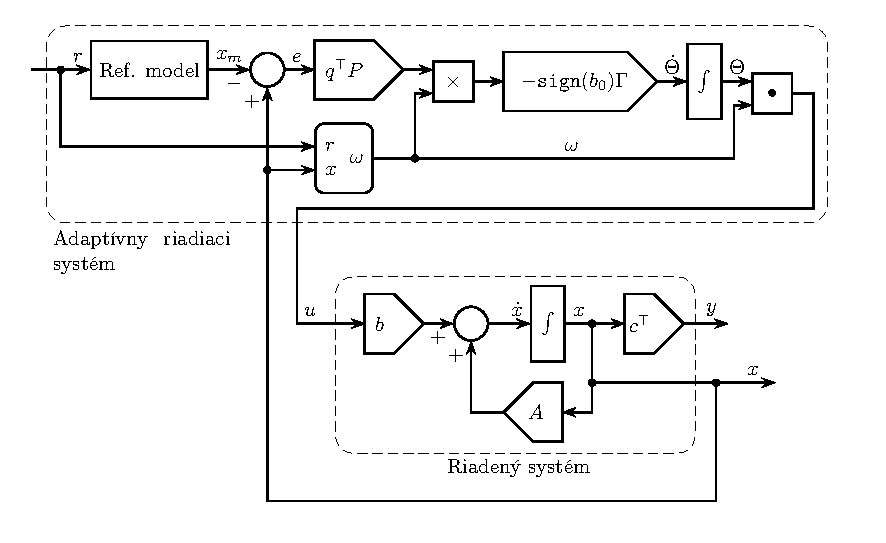
\includegraphics{Obr_ssARS_standalone.pdf}
	}
	\caption{Bloková schéma MRAC so stavovou štruktúrou riadenia} \label{Bloková schéma MRAC so stavovou štruktúrou riadenia}
\end{figure}






\begin{table}[b]
    \centering
    \catcode`\-=12
    \caption{MRAC so stavovou štruktúrou riadenia --- Zhrnutie}
    \label{MRAC so stavovou štruktúrou riadenia --- Zhrnutie}

    \begin{tabular*}{\textwidth}{  l  >{$\displaystyle}r<{$} @{$\,$} >{$\displaystyle}l<{$} }

        \toprule
        \multirow{2}{*}{Riadený systém}   &  \dot{x} = & A x + b u\\
                                          & y = & c^\naT	 x \\
        \midrule
        \multirow{2}{*}{Referenčný model} & \dot{x}_m =& A_m x_m + b_m r \\
                                          & y_m =&  c_m^\naT x_m \\
        \midrule
        Zákon riadenia & u = & k^\naT x + l r \\
        \midrule
        \multirow{2}{*}{Podmienky zhody}  & A_m =& A + b {k^\star}^\naT \\
                                          & b_m = & b l^\star \\
        \midrule
        Parametrizácia riadeného systému  & \dot{x} =& A_m x + b l^\star r + b \left( u - {k^\star}^\naT x - l^\star r \right) \\
        \midrule
        \multirow{2}{0.48\textwidth}{Dynamika adaptačnej odchýlky a~odchýlky parametrov zákona riadenia} & \dot{e} = & A_m e	+ b	\left( {\theta}^\naT \omega \right) \\
                                          & \dot{\theta} =& f \left( e, \omega \right) \\
        \midrule
        Zákon adaptácie & \dot{\Theta} = & - \texttt{sign}(b_0)	\Gamma e^\naT	P q \, \omega\\
        \bottomrule
    \end{tabular*}
\end{table}


%$












\subsection{Súhrn}

Zhrnutie návrhu Adaptívneho riadenia s~referenčným modelom so stavovou štruktúrou zákona riadenia je v~Tabuľke~\ref{MRAC so stavovou štruktúrou riadenia --- Zhrnutie}. Bloková schéma celého systému je na Obr.~\ref{Bloková schéma MRAC so stavovou štruktúrou riadenia}.











\section{Príklad: Systém 2. rádu vo všeobecnosti}


Uvažujme systém, ktorý je zadaný nasledujúcou sústavou rovníc
\begin{subequations} \label{system2radu_priklad}
\begin{align}
	\dot x_1 &= x_2  &  x_1(0) &=0 \\
	\dot x_2 &= -2 x_2 - x_1 + 0,5 u &  x_2(0)&=0 \\
	y &= x_1
\end{align}
\end{subequations}
Rovnice \eqref{system2radu_priklad} je možné zapísať v maticovom tvare:
\begin{subequations} \label{maticformasystemu2r_priklad}
	\begin{align}
	\begin{bmatrix}
	 		\dot x_1  \\
	 		\dot x_2
	 \end{bmatrix}
	 &=
	 \begin{bmatrix}
	 		0 & 1 \\
	 		-1 & -2
	 \end{bmatrix}
	 \begin{bmatrix}
	 		x_1  \\
	 		x_2
	 \end{bmatrix}
	 +
	 \begin{bmatrix}
	 		0  \\
	 		0,5
	 \end{bmatrix}
	 u
	 \\
	 y
	 &=
	 \begin{bmatrix}
	 		1  &
	 		0
	 \end{bmatrix}
	 \begin{bmatrix}
	 		x_1  \\
	 		x_2
	 \end{bmatrix}
	\end{align}
\end{subequations}
Ide o SISO systém 2. rádu, kde prvá stavová veličina je zároveň aj výstupnou veličinou a znamienko jediného nenulového prvku vektora $b$, teda parametra $b_0$ je $+$ (kladné).

Pre zadaný riadený systém navrhnime adaptívne riadenie s referenčným modelom so stavovou štruktúrou zákona riadenia, pričom referenčný model je v tvare
\begin{subequations}
	\begin{align}
	\begin{bmatrix}
	 		\dot x_{1m}  \\
	 		\dot x_{2m}
	 \end{bmatrix}
	 &=
	 \begin{bmatrix}
	 		0 & 1 \\
	 		-2 & -3
	 \end{bmatrix}
	 \begin{bmatrix}
	 		x_{1m}  \\
	 		x_{2m}
	 \end{bmatrix}
	 +
	 \begin{bmatrix}
	 		0  \\
	 		2
	 \end{bmatrix}
	 r
	 \label{stavovyOpisRM2R_priklad}
	\end{align}
\end{subequations}
Označme ako zvyčajne
	\begin{align*}
	 A
	 &=
	 \begin{bmatrix}
	 		0 & 1 \\
	 		-1 & -2
	 \end{bmatrix}
	 &
	 b
	 &=
	 \begin{bmatrix}
	 		0  \\
	 		0,5
	 \end{bmatrix}
	 &
	 A_m
	 &=
	 \begin{bmatrix}
	 		0 & 1 \\
	 		-2 & -3
	 \end{bmatrix}
	 &
	 b_m
	 &=
	 \begin{bmatrix}
	 		0  \\
	 		2
	 \end{bmatrix}
	\end{align*}
Je evidentné, že zákon riadenia -- stavový regulátor, má v tomto príklade tvar
\begin{equation} \label{stavZakRiad2r_priklad}
	u
	=
	\begin{bmatrix} k_1 & k_2 \end{bmatrix}
	\begin{bmatrix} x_1 \\ x_2 \end{bmatrix}
	+
	l \, r
\end{equation}
kde $k_1$, $k_2$, $l$ sú neznáme parametre regulátora (zosilnenia regulátora), ktoré sa budú adaptovať tak aby sa priebeh stavových veličín uzavretého regulačného obvodu zhodoval s priebehom stavových veličín referenčného modelu.

Ideálne parametre zákona riadenia sú
\begin{align}
    \begin{bmatrix} k_1^\star & k_2^\star \end{bmatrix}
    &=
    \texttt{pinv}(b) \left( A_m - A \right) = \begin{bmatrix} -2 & -2 \end{bmatrix}
    \\
    l^\star &= \texttt{pinv}(b) \, b_m = 4
\end{align}


Všeobecný tvar zákona adaptácie je
\begin{equation}
	\dot \Theta = - \texttt{sign}(b_0) \Gamma e^\naT P q \, \omega
\end{equation}
kde $P = P^\naT > 0$ spĺňa Lyapunovovu rovnicu $ A_m^\naT P + P A_m = - Q$ kde $Q = Q^\naT > 0$ je ľubovolná symetrická kladne definitná matica rovnakého rozmeru ako $A_m$. Zvoľme napríklad
\begin{align*}
	 Q &= \begin{bmatrix} 10 & 12,5\\ 12,5& 25 \end{bmatrix}
\end{align*}
Maticu $P$ získame riešením Lyapunovovej rovnice príkazom \textsc{Matlab}-u
\begin{equation}
	P = \texttt{lyap} \left( A_m^\naT, Q^\naT \right) = \begin{bmatrix} 5 &  2.5 \\   2,5  &  5 \end{bmatrix}
\end{equation}

Vektor $q$ má len posledný prvok rovný jednej, ostatné sú nulové, a rozmer má rovnaký ako vektor $b$, teda
\begin{equation}
	q = \begin{bmatrix} 0 \\ 1 \end{bmatrix}
\end{equation}

Výsledkom vynásobenia vektora signálov $e^\naT = \begin{bmatrix} e_1 & e_2 \end{bmatrix}$, matice $P$ a vektora $q$ je skalár (jednoducho signál s rozmerom $1 \times 1$), ktorý keď sa vynásobý so  signálnym vektorom $\omega$, ktorý obsahuje tri signály
\begin{equation}
	\omega = \begin{bmatrix} x_1 \\ x_2 \\ r \end{bmatrix}
\end{equation}
tak výsledkom je opäť stĺpcový vektor obsahujúci tri signály.

Adaptujeme tri parametre a výstupom zákona adaptácie sú derivácie týchto troch parametrov
\begin{equation}
	\dot \Theta = \begin{bmatrix} \dot{k}_1 \\ \dot{k}_2 \\ \dot{l} \end{bmatrix}
\end{equation}
Preto ak matica $\Gamma^{-1} = \left( \Gamma^{-1} \right)^\naT > 0$ je ľubovolná, \emph{diagonálna}, kladne definitná, potom je taká aj matica $\Gamma$ a v tomto prípade musí mať rozmer $3\times3$. Zvoľme
\begin{equation}
	\Gamma =
    \begin{bmatrix}
		1 & 0 & 0 \\
		0 & 1 & 0 \\
		0 & 0 & 1
	\end{bmatrix}
\end{equation}



Pre získanie okamžitých hodnôt parametrov zákona riadenia je potrebné integrovať výstup zákona adaptácie
\begin{equation}
	\Theta = \int \dot \Theta \, \textrm{d}t
\end{equation}
Integrátor môže mať nastavené tzv. začiatočné podmienky. V tomto prípade tieto predstavujú začiatočné hodnoty adaptovaných parametrov. Ak sú začiatočné hodnoty parametrov nastavené práve na ideálne (ktoré však vo všeobecnosti nepoznáme), priebeh stavových veličín riadeného systému hneď na začiatku spĺňa cieľ riadenia a~adaptácia nie je potrebná, teda výstupom zákona adaptácie bude nula -- čo zodpovedá tomu, že žiadna zmena (derivácia) parametrov regulátora nie je potrebná. Čím sú začiatočné hodnoty bližšie k ideálnym parametrom regulátora, tým skôr sa dosiahne cieľ riadenia.



































\section{Cvičenie piate}



\begin{enumerate}[leftmargin=0pt, labelsep=4mm, itemsep=0pt]

    \item Uvažujte model riadeného systému zadaný nasledovne
    \begin{subequations} \label{system3radu}
    \begin{align}
        \dot{x}_1 &= x_2   \\
        \dot{x}_2 &= x_3   \\
        \dot{x}_3 &= -2 x_3 + 3 x_2 - 20 x_1 + 50 u  \\
        y &= x_1
    \end{align}
    \end{subequations}
    so začiatočným stavom $x_1(0)=0$, $x_2(0)=0$, $x_3(0)=0$, kde $y(t)$ je výstupná veličina, $u(t)$ je vstupná veličina (akčný zásah) a $x_1(t)$, $x_2(t)$, $x_3(t)$ sú stavové veličiny.

    \begin{itemize}[leftmargin=0pt, labelsep=4mm, itemsep=0pt]

        \item Zapíšte systém v maticovom tvare
        \begin{subequations}
            \begin{align}
                 \dot x &= A x + b u \\
                 y &= c^\naT x
            \end{align}
        \end{subequations}

        \item Určte vstupno-výstupný opis riadeného systému -- prenosovú funkciu. 
        \item Určte nuly a póly systému a vyznačte ich v~komplexnej rovine. 
        \item Nakreslite blokovú schému systému (obsahujúcu stavové veličiny). 
        \item Vykreslite prechodovú charakteristiku systému, zároveň vykreslite priebehy stavových veličín (zostavte simulačnú schému, napríklad v Simulinku). 

    \end{itemize}





    \item Navrhnite stavový regulátor, taký, ktorý zabezpečí, že výsledný uzavretý regulačný obvod sa bude zhodovať s referenčným modelom v tvare
    \begin{subequations} \label{refmodelcv}
    \begin{align}
    	 \dot x_m &= A_m x_m + b_m r \\
    	 y_m &= c_m^\naT x_m
    \end{align}
    \end{subequations}

    \vspace{-2mm}

    \noindent
    kde
    \begin{align*}
        A_m
        &=
        \begin{bmatrix}
        		0 & 1 & 0 \\
        		0 & 0 & 1 \\
        		-5 & -11 & -7
        \end{bmatrix}
        &
        b_m &= \begin{bmatrix} 0 \\ 0 \\ 5 \end{bmatrix}
        &
        c_m &= \begin{bmatrix} 1 \\ 0 \\ 0 \end{bmatrix}
    \end{align*}

    \begin{itemize}[leftmargin=0pt, labelsep=4mm, itemsep=0pt]
        \item Určte počet parametrov spätnoväzbového člena a dopredného člena stavového regulátora a zapíšte zákon riadenia vo vektorovom tvare (bez číselných hodnôt parametrov).
        \item Určte vektor parametrov (celkový) $\Theta$ a signálny vektor $\omega$ zákona riadenia. 
        \item Určte podmienky zhody uzavretého regulačného obvodu a referenčného modelu. 
        \item Určte číselné hodnoty parametrov zákona riadenia (vyriešte podmienky zhody). 
        \item Zostavte simulačnú schému zákona riadenia a pridajte ju k simulačnej schéme riadeného systému. 
        \item Určte stavový opis URO, nuly a póly URO -- načrtnite ich v komplexnej rovine. 
        \item Vykreslite prechodovú charakteristiku URO (čo je „vstupom“ URO?) 
        \item Graficky porovnajte výstupy URO a RM. 
    \end{itemize}











    \begin{figure}[!t]
    	\centering

        % \vspace{-7mm}

    	\makebox[\textwidth][c]{%
    	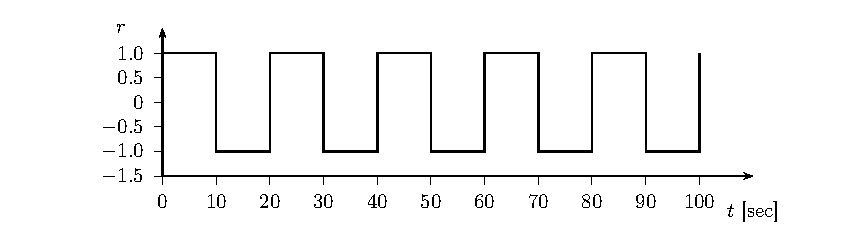
\includegraphics{Obr_cv3Vzor_1.pdf}
    	}

        \vspace{-5mm}

    	\caption{Referenčný signál $r$}
    	\label{Referenčný sigál $r$ 4cv}

        % \vspace{-7mm}

    \end{figure}





    % \begin{figure}[!t]
    % 	\centering

    % 	\makebox[\textwidth][c]{%
    % 	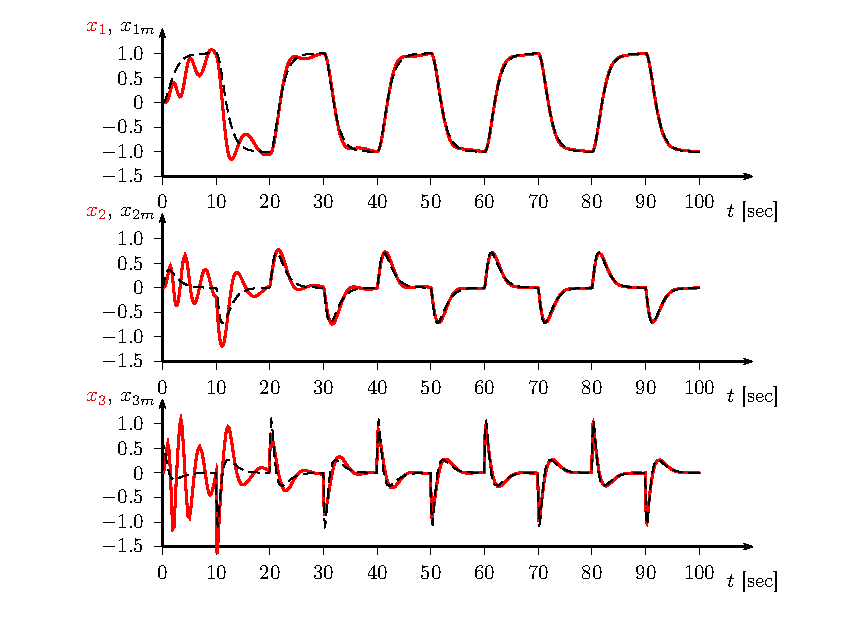
\includegraphics{Obr_cv3Vzor_2.pdf}
    % 	}

    %     \vspace{-7mm}

    % 	\caption{Výsledok simulácie}
    % 	\label{Výsledok simulácie 4cv}

    %     \vspace{-5mm}

    % \end{figure}








    \item V ďalšom predpokladajte, že nie všetky parametre systému sú známe. Známa nech je len štruktúra systému (rozmery matíc $A$, $b$, $c$), že ide o SISO systém, že nenulový prvok matice $c$ je rovný jednotke, a~že prvá stavová veličina je zároveň aj výstupnou veličinou, a~tiež nech je známa pozícia a znamienko jediného nenulového prvku vektora $b$. Stavový vektor riadeného systému je merateľný.

    Pre zadaný riadený systém navrhnite adaptívne riadenie s referenčným modelom so stavovou štruktúrou zákona riadenia. Pre odvodenie zákona adaptácie použite priamu Lyapunovou metódu. Referenčný model nech je v tvare \eqref{refmodelcv}.

    \begin{itemize}[leftmargin=0pt, labelsep=4mm, itemsep=0pt]
    	\item Z predchádzajúcej úlohy formálne modifikujte zákon riadenia, ktorý sa bude používať v adaptívnom riadiacom systéme.
    	\item Ukážte existenciu ideálnych parametrov zákona riadenia. 
    	\item Stanovte diferenciálnu rovnicu, ktorá dáva do vzťahu adaptačnú odchýlku a chybu nastavenia parametrov zákona riadenia. 
    	\item Určte zákon adaptácie, ktorý sa bude používať v adaptívnom riadiacom systéme.
        \begin{itemize}[leftmargin=0pt, labelsep=4mm, itemsep=0pt] 
            \item Pre systém diferenciálnych rovníc ($\dot e, \dot \theta$), kde $\dot \theta$ sa najskôr uvažuje vo všeobecnom tvare (na začiatku odvodenia sa uvažuje len všeob. funkcia $f$) zvoľte kandidáta na Lyapunovovu funkciu a odvoďte (skonkretizujte) predpis (pravú stranu) pre $\dot \theta$.
            \item Zvoľte $Q$ a vypočítajte $P$ (alebo len určte $P$).
        	\item Zvoľte $\Gamma$. 
        \end{itemize}
    	\item Začiatočné hodnoty adaptovaných parametrov zvoľte nulové.
    	\item Zostavte adaptívny riadiaci systém (simulačnú schému) a pridajte ho k~simulovanému riadenému systému. 
    	\item Demonštrujte funkčnosť adaptívneho riadiaceho systému. Použite obdĺžnikový referenčný signál $r$ ako na Obr.~\ref{Referenčný sigál $r$ 4cv}. 
        % Vzorové výsledky simulácie sú na Obr.~\ref{Výsledok simulácie 4cv}. 

    \end{itemize}


\end{enumerate}




























\section{Príklad: Kyvadlo}



\subsection{Celkový pohľad na úlohu}

Nech riadeným systémom je kyvadlo a nech riadenou veličinou je poloha (uhol) kyvadla. Zároveň, nech riadený systém je daný diferenciálnou rovnicou opisujúcu dynamiku rotačného pohybu kyvadla. Rovnica je v tvare
\begin{equation} \label{analOpRS}
    ml^2 \ddot{\varphi}(t) + \beta \dot{\varphi}(t) + mgl\sin{\varphi(t)} = u(t)
\end{equation}
kde hmotný bod s hmotnosťou $m$ [kg] pripevnený na ramene so zanedbateľnou hmotnosťou a dĺžkou $l$ [m] kmitá (otáča sa okolo osi). Kmity sú tlmené viskóznym trením s koeficientom $\beta$ [kg m$^2$ s$^{-1}$]. Uhol medzi zvislicou a ramenom kyvadla je označený $\varphi$ [rad] a gravitačné zrýchlenie je $g = 9,81$ [m s$^{-2}$]. Signál $u(t)$ [kg m$^2$ s$^{-2}$] je externý moment sily pôsobiaci na rameno kyvadla, $\dot{\varphi}(t)$ [rad s$^{-1}$] je uhlová rýchlosť a $\ddot{\varphi}(t)$ [rad s$^{-2}$] je uhlové zrýchlenie ramena kyvadla.
Číselné hodnoty parametrov kyvadla sú nasledovné:
\begin{align*}
	m &= 1 \quad \text{[kg]}\\
	l &= 1 \quad \text{[m]}\\
	\beta &= 2 \cdot 0,5 \cdot \sqrt{\frac{g}{l}} \quad \text{[kg m$^2$ s$^{-1}$]}
\end{align*}

Cieľom je riadiť polohu kyvadla v okolí rôznych pracovných bodov. Uvažujme však, že pracovné body sú z intervalu polôh kyvadla 0 až 90 stupňov. Konkrétna voľba pracovných bodov ako aj voľba veľkosti ich okolia sa ponechávajú na čitateľa.






\subsection{Riadený systém (z hľadiska návrhu riadiaceho systému)}




Pre lepšiu predstavu o riadenom systéme ho opíšme v stavovom priestore. Voľbou stavových veličín $x_1(t) = \varphi(t)$ a~$x_2(t) = \dot\varphi(t)$ máme
\begin{subequations} \label{stavopnonlinkyv}
	\begin{align}
		\begin{bmatrix}
			\dot{x}_1(t) \\ \dot{x}_2(t)
		\end{bmatrix}
		&=
		\begin{bmatrix}
			x_2(t) \\ - \frac{\beta}{ml^2} x_2(t) - \frac{g}{l} \sin\left(x_1(t)\right)
		\end{bmatrix}
		+
		\begin{bmatrix}
			0 \\ \frac{1}{ml^2}
		\end{bmatrix}
		u(t) \\
		y(t) &= x_1(t)
	\end{align}
\end{subequations}
kde sme pre prehľadnosť v nasledujúcom zaviedli aj výstupnú veličinu $y(t) = \varphi(t)$.


Toto je, zjavne, nelineárny časovo-invariantný systém druhého rádu. Tu sa však zaoberáme takou triedou riadiacich systémov, ktoré predpokladajú lineárny model riadeného systému. Jeho parametre môžu byť neznáme (môžu sa meniť), ale musí byť lineárny.

\paragraph{Linearizácia v okolí pracovného bodu}

Uvažovaný riadený systém je možné linearizovať v okolí pracovného bodu.

V prvom rade potrebujeme poznať pracovný bod. Pre zvolenú hodnotu (ustálenú) na vstupe systému, označme ju $u_{PB}$, potrebujeme poznať prislúchajúcu hodnotu (ustálenú) na výstupe, označme ju $y_{PB}$.

Tu máme k dispozícii analytický opis riadeného systému \eqref{analOpRS}. V ustálenom stave (časové derivácie nulové) máme
\begin{subequations}
    \begin{align}
        \left(m g l\right)\sin\left(y_{PB}\right) &= u_{PB} \\
         y_{PB} &= \arcsin \left( \frac{1}{ \left(m g l\right)} u_{PB} \right)
    \end{align}
\end{subequations}
Toto je, samozrejme, prevodová charakteristika riadeného systému. Nie je to priamka. To znamená, že v jednom pracovnom bode (v okolí jedného pracovného bodu) bude statické zosilnenie (sklon prevodovej charakteristiky) iné, ako v inom pracovnom bode (v okolí iného pracovného bodu).

\bigskip

Mimochodom, zvoľme si veľkosť okolia pracovného bodu. Dobrou pomôckou je grafické zobrazenie prevodovej charakteristiky. To sa ponecháva na čitateľa (autor je lenivý). Tu si zvoľme okolie z veľkosťou $\pm 3$ [°] (cca $0,0524$ [rad]) na strane výstupnej veličiny a~buďme s ním spokojný v tom zmysle, že pri takýchto malých odchýlkach si prevodová charakteristika zachováva prakticky rovnaký sklon ako v pracovnom bode.

\bigskip

Ďalej je potrebné zaviesť veličiny, ktoré budú takpovediac odchýlkami od hodnôt v pracovnom bode. Konkrétne
\begin{subequations}
    \begin{align}
        \Delta u(t) &= u(t) - u_{PB} \\
        \Delta y(t) &= y(t) - y_{PB}
    \end{align}
\end{subequations}
kde sme teta definovali $\Delta$ odchýlky od pracovného bodu. To znamená, že pôvodné veličiny sú
\begin{subequations}
    \begin{align}
        u(t)  &=  u_{PB} + \Delta u(t) \\
        y(t)  &=  y_{PB} + \Delta y(t) \\
        x_1(t)  &=  x_{1PB} + \Delta x_1(t) \\
        x_2(t)  &=  x_{2PB} + \Delta x_2(t)
    \end{align}
\end{subequations}
kde sme rovnako zaviedli „odchýlkové veličiny“ aj pre stavové veličiny so systému \eqref{stavopnonlinkyv}. Vzhľadom na takto uvedený pracovný bod je možné analyticky linearizovať dynamický systém \eqref{stavopnonlinkyv} s využitím rozvoja funkcie do Taylorovho radu.

Vo všeobecnosti, autonómny dynamický systém je
\begin{align}
    \dot x = F(x)
\end{align}
kde funkcia $F(x)$ je, vo všeobecnosti, nelineárna. V pracovnom bode $x_{PB}$, pričom $x = x_{PB} + \Delta x$ a $\Delta x$ je odchýlka od bodu $x_{PB}$, v tomto pracovnom bode je možné aproximovať funkciu $F(x)$ prvými dvomi členmi Taylorovho rozvoja, teda
\begin{align}
    F(x) = F(x_{PB} + \Delta x) \approx F(x_{PB}) +   \left. \frac{\partial F(x)}{\partial x} \right|_{x=x_{PB}}\Delta x
\end{align}

Obdobne, ak by sme mali neautonómny dynamický systém
\begin{align}
    \dot x = F(x, u)
\end{align}
kde $u$ je vstupný signál systému, tak aproximácia v zmysle Taylorovho rozvoja by bola
\begin{align}
    F(x, u) 
    \approx F(x_{PB}, u_{PB}) 
    + \left. \frac{\partial F(x,u)}{\partial x} \right|_{x=x_{PB}}\Delta x
    + \left. \frac{\partial F(x,u)}{\partial u} \right|_{u=u_{PB}}\Delta u
\end{align}
kde sme samozrejme zaviedli $u = u_{PB} + \Delta u$ tak ako pri $x$.

Konečne, pre prípad kyvadla môžme o \eqref{stavopnonlinkyv} uvažovať ako o dvoch funkciách takých, že
\begin{align}
    \dot x_1 &= F_1(x_1, x_2, u) = x_2 \\
    \dot x_2 &= F_2(x_1, x_2, u) = - \frac{\beta}{ml^2} x_2 - \frac{g}{l} \sin\left(x_1\right) + \frac{1}{ml^2} u
\end{align}
Ich aproximácie potom sú
\begin{align}
    F_1 
    &\approx F_1(x_{1PB}, x_{2PB}, u_{PB}) 
    + \left. \frac{\partial F_1}{\partial x_1} \right|_{x_{1PB}}\Delta x_1
    + \left. \frac{\partial F_1}{\partial x_2} \right|_{x_{2PB}}\Delta x_2
    + \left. \frac{\partial F_1}{\partial u} \right|_{u_{PB}}\Delta u
    \\
    F_2 
    &\approx F_2(x_{1PB}, x_{2PB}, u_{PB}) 
    + \left. \frac{\partial F_2}{\partial x_1} \right|_{x_{1PB}}\Delta x_1
    + \left. \frac{\partial F_2}{\partial x_2} \right|_{x_{2PB}}\Delta x_2
    + \left. \frac{\partial F_2}{\partial u} \right|_{u_{PB}}\Delta u
\end{align}

Konkretizujme jednotlivé výrazy. Vzhľadom na to, že pracovný bod je bodom na prevodovej charakteristike, tak
\begin{align}
    F_1(x_{1PB}, x_{2PB}, u_{PB}) &= 0 \\
    F_2(x_{1PB}, x_{2PB}, u_{PB}) &= 0 
\end{align}
a ďalej
\begin{align}
    \left. \frac{\partial F_1}{\partial x_1} \right|_{x_1=x_{1PB}} &= 0 &
    \left. \frac{\partial F_1}{\partial x_2} \right|_{x_2=x_{2PB}} &= 1 &
    \left. \frac{\partial F_1}{\partial u} \right|_{u=u_{PB}} &= 0 \\
    \left. \frac{\partial F_2}{\partial x_1} \right|_{x_1=x_{1PB}} &= - \frac{g}{l} \cos\left(x_{1PB}\right) &
    \left. \frac{\partial F_2}{\partial x_2} \right|_{x_2=x_{2PB}} &= - \frac{\beta}{ml^2} &
    \left. \frac{\partial F_2}{\partial u} \right|_{u=u_{PB}} &=  \frac{1}{ml^2}
\end{align}
Preto
\begin{align}
    F_1(x_1, x_2, u) &\approx \Delta x_2 \\
    F_2(x_1, x_2, u) &\approx  - \frac{g}{l} \cos\left(x_{1PB}\right) \Delta x_1   - \frac{\beta}{ml^2} \Delta x_2 + \frac{1}{ml^2} \Delta u
\end{align}
K tomu ak uvážime, že ľavú strana rovnice \eqref{stavopnonlinkyv} je možné písať ako
% \begin{subequations}
	\begin{align}
		\begin{bmatrix}
			\frac{\text{d}}{\text{d}t} \left( x_{1PB} + \Delta x_1(t) \right)   \\
            \frac{\text{d}}{\text{d}t} \left( x_{2PB} + \Delta x_2(t) \right)
		\end{bmatrix}
        =
        \begin{bmatrix}
			 \Delta \dot x_1(t)    \\
             \Delta \dot x_2(t)
		\end{bmatrix}
	\end{align}
% \end{subequations}
pretože $x_{1PB}$ a $x_{2PB}$ sú len čísla nezávislé od času, tak s aproximáciami funkcií $F_1(x_1, x_2, u)$ a $F_2(x_1, x_2, u)$ prejde \eqref{stavopnonlinkyv} do tvaru
\begin{subequations} %\label{stavopnonlinkyv2}
	\begin{align}
        \Delta \dot x_1(t) &=  \Delta x_2(t) \\
        \Delta \dot x_2(t) &=
        - \frac{g}{l} \cos\left(x_{1PB}\right) \Delta x_1   - \frac{\beta}{ml^2} \Delta x_2 + \frac{1}{ml^2} \Delta u \\
        \Delta y(t) &= \Delta x_1(t)
	\end{align}
\end{subequations}
kde sme zohľadnili, že musí platiť $\Delta y(t) = \Delta x_1(t)$, keďže máme $y(t) = x_1(t)$. Tento dynamický systém je možné zapísať aj v maticovom tvare
\begin{subequations} \label{stavoplinkyv}
    \begin{align}
    	\begin{bmatrix}
        	  \Delta \dot x_1(t) \\
    		  \Delta \dot x_2(t)
     	\end{bmatrix}
    	&=
    	\begin{bmatrix}
        	0 & 1 \\
        	- \frac{g}{l} \cos \left( y_{PB} \right) & - \frac{\beta}{m\ l^2}
      	\end{bmatrix}
        \begin{bmatrix}
        	  \Delta x_1(t) \\
    		  \Delta x_2(t)
     	\end{bmatrix}
        +
        \begin{bmatrix}
        	  0 \\
    		  \frac{1}{m\ l^2}
     	\end{bmatrix}
        \Delta u(t)
        \\
        \Delta y(t)
        &=
        \begin{bmatrix}
            1 & 0 \\
        \end{bmatrix}
        \begin{bmatrix}
              \Delta x_1(t) \\
              \Delta x_2(t)
        \end{bmatrix}
    \end{align}
\end{subequations}
Toto je lineárny dynamický systém, ktorý je možné zapísať v tvare prenosovej funkcie
\begin{align}
    \frac{\Delta y(s)}{\Delta u(s)} = \frac{b_0}{s^2 + a_1 s + a_0}
\end{align}
kde
\begin{subequations}
    \begin{align}
        b_0 &= \frac{1}{m\ l^2} \\
        a_0 &= \frac{g}{l} \cos \left( y_{PB} \right) = \frac{g}{l} \cos \left( \arcsin \left( \frac{1}{ \left(m g l\right)} u_{PB} \right) \right) \\
        a_1 &= \frac{\beta}{m\ l^2}
    \end{align}
\end{subequations}
Je teda zrejmé, že statické a dynamické vlastnosti tohto lineárneho systému sú závislé od pracovného bodu.









\paragraph{Ilustrácia potreby adaptácie}







Z uvedeného je zrejmé, že statické a dynamické vlastnosti tohto lineárneho systému sú závislé od pracovného bodu. Ak by sme navrhli riadiaci systém, tak, že sa splní cieľ riadenia v okolí jedného pracovného bodu, potom v inom pracovnom bode (v jeho okolí) by tento nespĺňal cieľ riadenia.

Ukážme zmenu vlastností (statických aj dynamických) rideného systému (nelineárneho kavydla), tak, že budeme robiť skokové zmeny v okolí jedného pracovného bodu, a potom v okolí iného pracovného bodu.

Zvoľme pracovné body
\begin{subequations}
    \begin{align}
        u_{PB1} &= 5 &       y_{PB1} &= 0,5348 \ \text{[rad]} = 30,64 \ \text{[deg]}\\
        u_{PB2} &= 9 &       y_{PB2} &= 1,1616 \ \text{[rad]} = 66,55 \ \text{[deg]}
    \end{align}
\end{subequations}

Pre prvý praconý bod $\left( u_{PB1}, y_{PB1} \right)$ vypočítajme aj parametre lineárneho modelu (platného len v okolí pracovného bodu)
\begin{subequations} \label{parsysdemo}
    \begin{align}
        b_0 &= 1 \\
        a_0 &= 8,44 \\
        a_1 &= 3,13
    \end{align}
\end{subequations}



Simulujme teraz aj nelineárny systém, aj lineárny systém (celý čas s parametrami \eqref{parsysdemo}), pričom vstupom nech sú skokové zmeny v okolí zvolených pracovných bodov. Výsledok je na obr.~\ref{figsc_ar05_Kyvadlo_ep1_1}.




\begin{figure}[!t]
	\centering

    \vspace{-3mm}

	\makebox[\textwidth][c]{%
	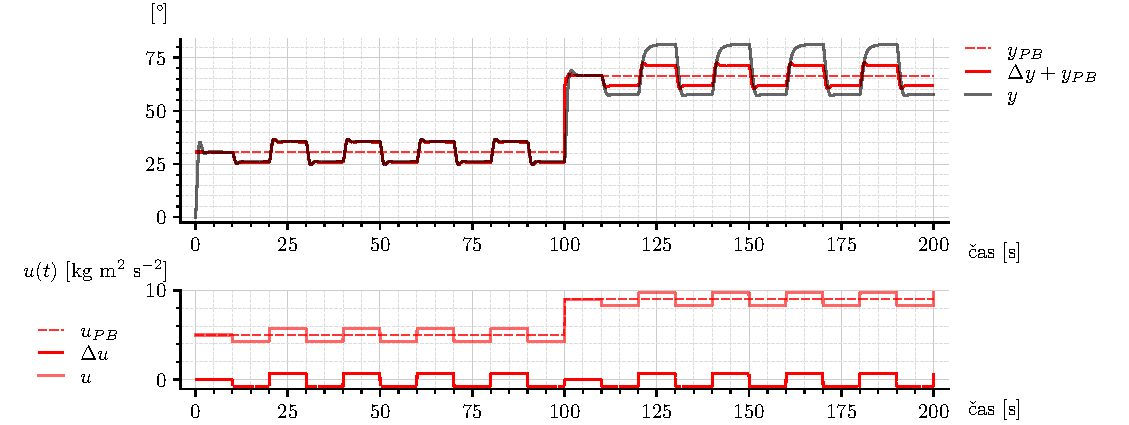
\includegraphics{figsc_ar05_Kyvadlo_ep1_1.pdf}
	}

    \vspace{-2mm}

	\caption{Porovnanie výstupov lineárneho a nelineárneho systému v okolí rôznych pracovných bodov.}
	\label{figsc_ar05_Kyvadlo_ep1_1}

    \vspace{-2mm}

\end{figure}



% V prvom pracovnom bode sa lineárny a nelineárny systém zhodujú ale v druhom už nie. Aby sa zhodoval, musel by lineárny model zmeniť (prispôsobiť) parametre.  Inými slovami, parametre modelu riadeného systému sa menia v závislosti od pracovného bodu. Preto je potrebné mať adaptívny riadiaci systém\ldots






\paragraph{Dostupnosť stavových veličín}

Zároveň si vzhľadom na uvedené dovoľujeme zdôrazniť dostupnosť stavových veličín pre spätnú väzbu. Stavovými veličinami sú poloha a rýchlosť kyvadla. Jednoznačne ide o veličiny, ktoré je možné merať. Pre simuláciu na obr.~\ref{figsc_ar05_Kyvadlo_ep1_1} uvádzame aj explicitné vykreslenie priebehu stavových veličín -- viď. obr.~\ref{figsc_ar05_Kyvadlo_ep1_ss_1}






\begin{figure}[!b]
	\centering

    \vspace{-3mm}

	\makebox[\textwidth][c]{%
	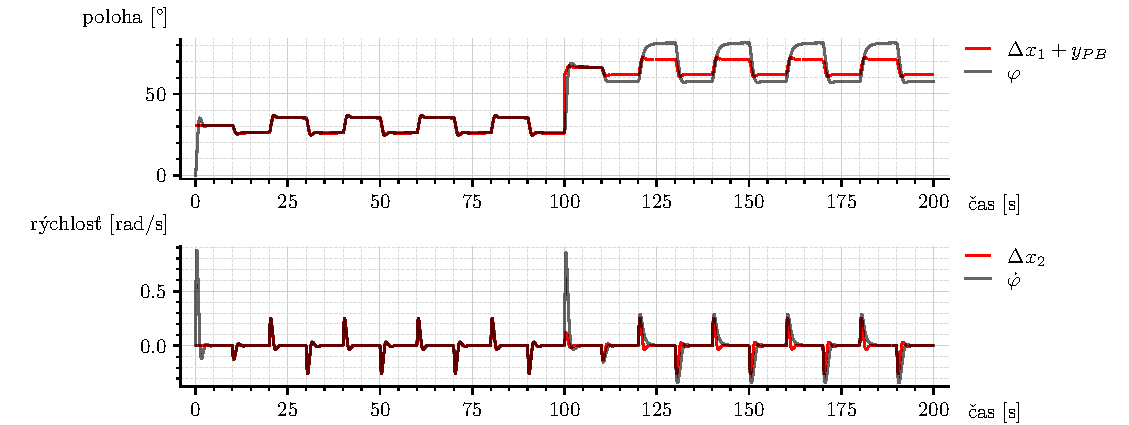
\includegraphics{figsc_ar05_Kyvadlo_ep1_ss_1.pdf}
	}

    \vspace{-2mm}

	\caption{Porovnanie výstupov lineárneho a nelineárneho systému v okolí rôznych pracovných bodov.}
	\label{figsc_ar05_Kyvadlo_ep1_ss_1}

    \vspace{-2mm}

\end{figure}







\subsection{Návrh adaptívneho riadiaceho systému}

Model riadeného systému sa uvažuje v tvare \eqref{stavoplinkyv}. Ide o SISO systém 2. rádu, kde prvá stavová veličina je zároveň aj výstupnou veličinou a znamienko jediného nenulového prvku vektora $b$, teda parametra $b_0$, je $+$ (kladné). Na parametre riadeného systému opísaného v stavovom priestore sa tu budeme odvolávať klasickým označovaním $A$, $b$ a prípadne $c^\naT$.



Pre uvedený riadený systém navrhnime adaptívne riadenie s referenčným modelom so stavovou štruktúrou zákona riadenia, pričom referenčný model nech je v tvare
\begin{subequations}
	\begin{align}
	\begin{bmatrix}
	 		\dot x_{1m}  \\
	 		\dot x_{2m}
	 \end{bmatrix}
	 &=
	 \begin{bmatrix}
	 		0 & 1 \\
	 		-2 & -3
	 \end{bmatrix}
	 \begin{bmatrix}
	 		x_{1m}  \\
	 		x_{2m}
	 \end{bmatrix}
	 +
	 \begin{bmatrix}
	 		0  \\
	 		2
	 \end{bmatrix}
	 r
	 \label{stavovyOpisRM2R_priklad2}
	\end{align}
\end{subequations}



Je zrejmé, že zákon riadenia má v tomto príklade tvar
\begin{equation} \label{stavZakRiad2r_priklad2}
	u
	=
	\begin{bmatrix} k_1 & k_2 \end{bmatrix}
	\begin{bmatrix} x_1 \\ x_2 \end{bmatrix}
	+
	l \, r
\end{equation}
kde $k_1$, $k_2$, $l$ sú neznáme parametre regulátora (zosilnenia regulátora), ktoré sa budú adaptovať tak aby sa priebeh stavových veličín uzavretého regulačného obvodu zhodoval s priebehom stavových veličín referenčného modelu.

Ideálne parametre zákona riadenia sú vo všeobecnosti
\begin{align}
    \begin{bmatrix} k_1^\star & k_2^\star \end{bmatrix}
    &=
    \texttt{pinv}(b) \left( A_m - A \right)
    \\
    l^\star &= \texttt{pinv}(b)
\end{align}





Všeobecný tvar zákona adaptácie je
\begin{equation}
	\dot \Theta = - \texttt{sign}(b_0) \Gamma e^\naT P q \, \omega
\end{equation}
kde $P = P^\naT > 0$ spĺňa Lyapunovovu rovnicu $ A_m^\naT P + P A_m = - Q$ kde $Q = Q^\naT > 0$ je ľubovoľná symetrická kladne definitná matica rovnakého rozmeru ako $A_m$. Zvoľme napríklad
\begin{align*}
	 Q &= \begin{bmatrix} 1 & 0\\ 0& 1 \end{bmatrix}
\end{align*}
Maticu $P$ získame riešením Lyapunovovej rovnice nástrojom z Python knižnice SciPy, metódou \lstinline{linalg.solve_continuous_lyapunov()}. Výsledok:
\begin{equation}
	P = \begin{bmatrix} 1,25 &  0,25 \\   0,25  &  0,25 \end{bmatrix}
\end{equation}

Vektor $q$ má len posledný prvok rovný jednej, ostatné sú nulové, a rozmer má rovnaký ako vektor $b$, teda
\begin{equation}
	q = \begin{bmatrix} 0 \\ 1 \end{bmatrix}
\end{equation}

Výsledkom vynásobenia vektora signálov $e^\naT = \begin{bmatrix} e_1 & e_2 \end{bmatrix}$, matice $P$ a vektora $q$ je skalár (jednoducho signál s rozmerom $1 \times 1$), ktorý keď sa vynásobý so  signálnym vektorom $\omega$, ktorý obsahuje tri signály
\begin{equation}
	\omega = \begin{bmatrix} x_1 \\ x_2 \\ r \end{bmatrix}
\end{equation}
tak výsledkom je opäť stĺpcový vektor obsahujúci tri signály.

Adaptujeme tri parametre a výstupom zákona adaptácie sú derivácie týchto troch parametrov
\begin{equation}
	\dot \Theta = \begin{bmatrix} \dot{k}_1 \\ \dot{k}_2 \\ \dot{l} \end{bmatrix}
\end{equation}
Preto ak matica $\Gamma^{-1} = \left( \Gamma^{-1} \right)^\naT > 0$ je ľubovolná, \emph{diagonálna}, kladne definitná, potom je taká aj matica $\Gamma$ a v tomto prípade musí mať rozmer $3\times3$. Zvoľme
\begin{equation}
	\Gamma =
    \begin{bmatrix}
		24000 & 0 & 0 \\
		0 & 400 & 0 \\
		0 & 0 & 12000
	\end{bmatrix}
\end{equation}



Pre získanie okamžitých hodnôt parametrov zákona riadenia je potrebné integrovať výstup zákona adaptácie
\begin{equation}
	\Theta = \int \dot \Theta \, \textrm{d}t
\end{equation}




\subsubsection{Vytvorenie predstavy o nastavení rýchlosti adaptácie}


Majme nejakú predstavu o riadenom systéme. V realite azda vždy budeme mať. Tu sa to teraz myslí, tak, že máme aspoň nejakú predstavu o parametroch lineárneho modelu skutočného riadeného systému (nelineárneho kyvadla). Použime tie isté parametre, aké sme už použili pre ilustračné účely, teda hodnoty parametrov \eqref{parsysdemo}. Zostavme simulačnú schému MRAC stavového avšak s tým, že riadeným systémom je priamo tento lineárny model. Umožní nám to vytvoriť si predstavu o tom, ako zvoliť maticu $\Gamma$ tak, aby rýchlosť adaptácie bola prijateľná.

Pre začiatok, uvažujme všetky váhy (prvky na diagonále) v $\Gamma$ rovnaké, o veľkosti „aby sa niečo dialo“. V tomto prípade je to
\begin{equation*}
    \Gamma = \texttt{diag}
    \left(
    \begin{bmatrix}
        1000 & 1000 & 1000
    \end{bmatrix}
    \right)
\end{equation*}
a zároveň uvažujeme harmonický signál s relatívne nízkou frekvenciou pre najjednoduchší možný prípad čo sa „obtiažnosti adaptácie“ týka. Výsledok je na obr.~\ref{figsc_ar05_Kyvadlo_ep2_1}.




\begin{figure}[!t]
	\centering

    \vspace{-3mm}

	\makebox[\textwidth][c]{%
	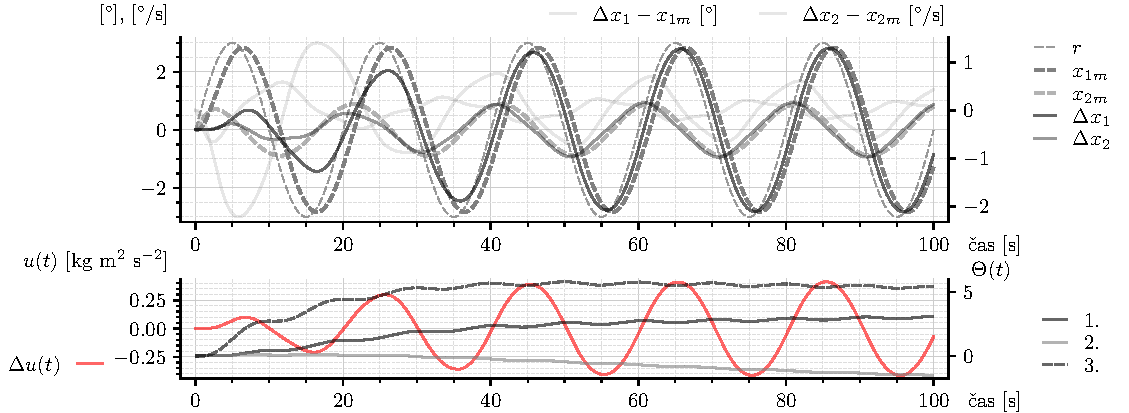
\includegraphics{figsc_ar05_Kyvadlo_ep2_1.pdf}
	}

    \vspace{-2mm}

	\caption{}
	\label{figsc_ar05_Kyvadlo_ep2_1}

    \vspace{-2mm}

\end{figure}




\begin{figure}[!b]
	\centering

    \vspace{-3mm}

	\makebox[\textwidth][c]{%
	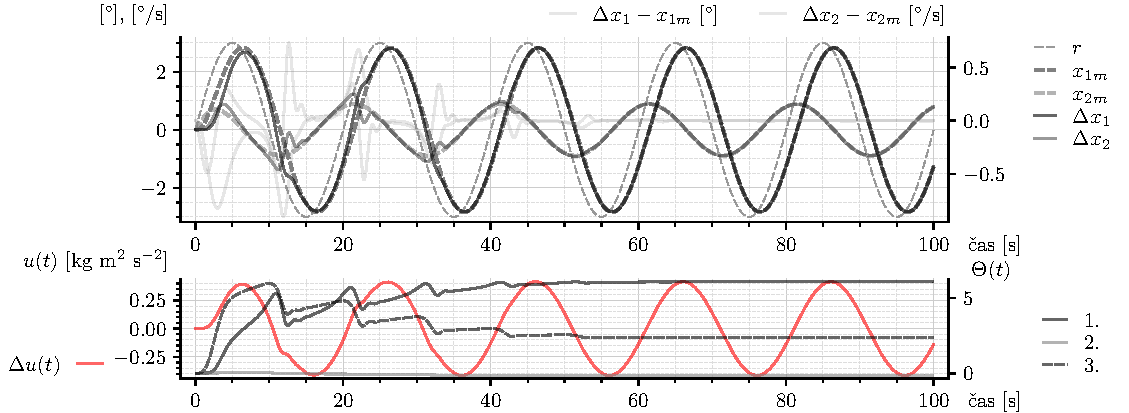
\includegraphics{figsc_ar05_Kyvadlo_ep2_2.pdf}
	}

    \vspace{-2mm}

	\caption{}
	\label{figsc_ar05_Kyvadlo_ep2_2}

    \vspace{-2mm}

\end{figure}




Je zrejmé, že je potrebné ladiť $\Gamma$ tak, aby rýchlosť zmeny adaptovaných parametrov (alebo aspoň väčšiny z nich) bola (aspoň na začiatku) čo najviac rovnaká. Po chvíli experimentovania sa dá dospieť k voľbe
\begin{equation*}
    \Gamma = \texttt{diag}
    \left(
    \begin{bmatrix}
        24000      & 400 & 12000
    \end{bmatrix}
    \right)
\end{equation*}
ako sme už uviedli, a výsledok je na obr.~\ref{figsc_ar05_Kyvadlo_ep2_2}.

Toto je už uspokojivý priebeh adaptovaných parametrov čo sa rýchlosti adaptácie týka.

Fungovalo by toto nastavenie aj pre iný priebeh referenčného signálu? Viď výsledok na obr.~\ref{figsc_ar05_Kyvadlo_ep2_3}. Kupodivu fungovalo.






\begin{figure}[!t]
	\centering

    \vspace{-3mm}

	\makebox[\textwidth][c]{%
	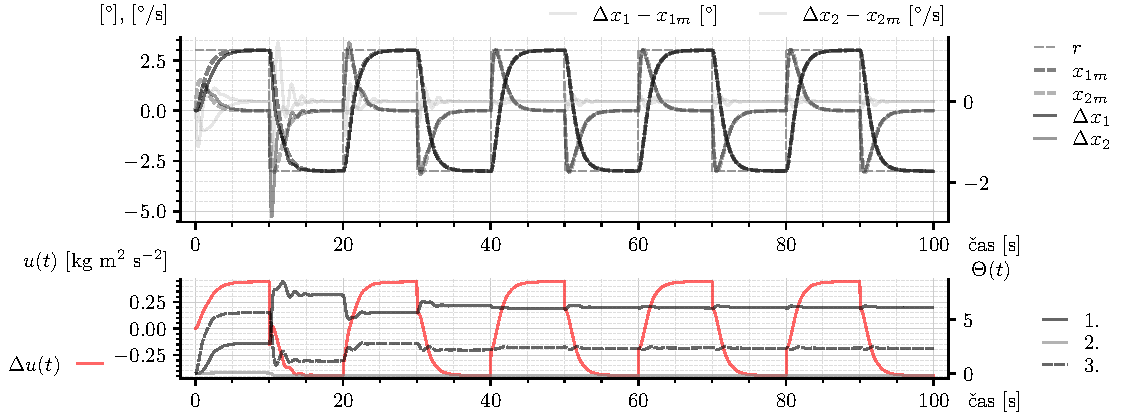
\includegraphics{figsc_ar05_Kyvadlo_ep2_3.pdf}
	}

    \vspace{-2mm}

	\caption{}
	\label{figsc_ar05_Kyvadlo_ep2_3}

    \vspace{-2mm}

\end{figure}



\subsection{Nasadenie na uvažovaný nelineárny systém}

Fungovalo by toto riadenie aj keby bolo nasadené na nelineárny systém? Teda priamo na nelineárne kyvydlo? Vyskúšajme - viď obr.~\ref{figsc_ar05_Kyvadlo_ep3_1}.





\begin{figure}[!b]
	\centering

    \vspace{-3mm}

	\makebox[\textwidth][c]{%
	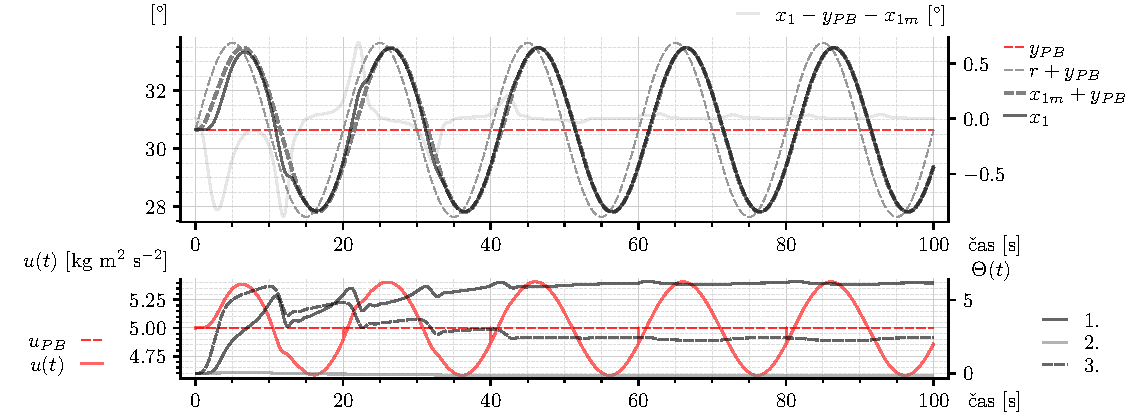
\includegraphics{figsc_ar05_Kyvadlo_ep3_1.pdf}
	}
    \makebox[\textwidth][c]{%
	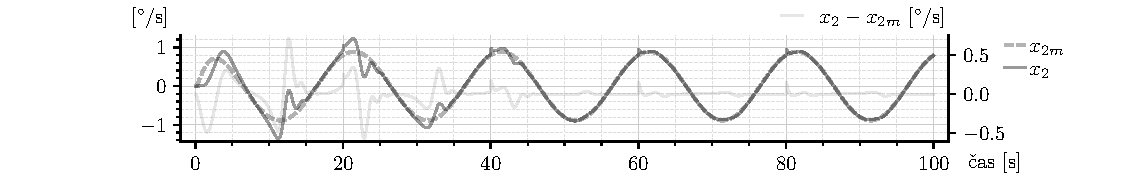
\includegraphics{figsc_ar05_Kyvadlo_ep3_x2_1.pdf}
	}

    \vspace{-2mm}

	\caption{}
	\label{figsc_ar05_Kyvadlo_ep3_1}

    \vspace{-2mm}

\end{figure}




Fungovalo\ldots Aj pre obdĺžnikový referenčný signál? Fungovalo\ldots viď obr.~\ref{figsc_ar05_Kyvadlo_ep3_2}.



\begin{figure}[!t]
	\centering

    \vspace{-3mm}

	\makebox[\textwidth][c]{%
	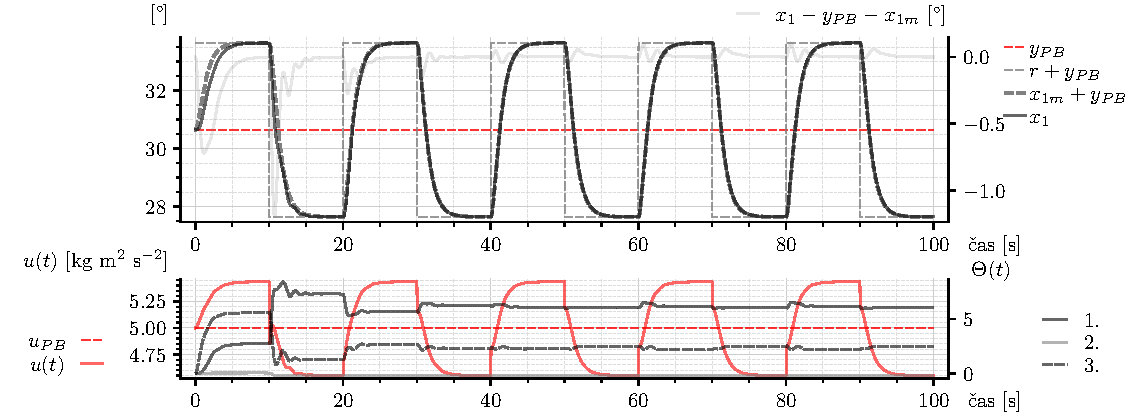
\includegraphics{figsc_ar05_Kyvadlo_ep3_2.pdf}
	}
    \makebox[\textwidth][c]{%
	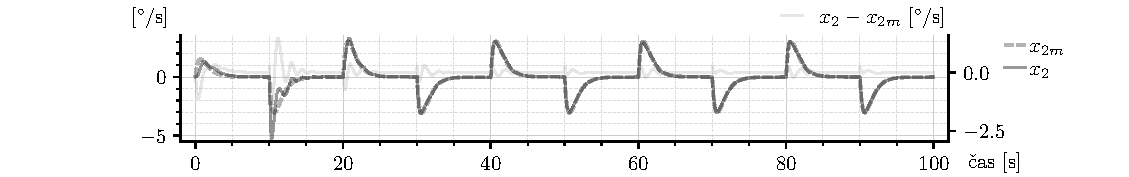
\includegraphics{figsc_ar05_Kyvadlo_ep3_x2_2.pdf}
	}

    \vspace{-2mm}

	\caption{}
	\label{figsc_ar05_Kyvadlo_ep3_2}

    \vspace{-2mm}

\end{figure}





Vyskúšajme teraz simuláciu, kde v čase 100 zmeníme pracovný bod na hodnotu $u_{PB} = 6$ (z pôvodnej hodnoty $u_{PB} = 5$), necháme ustáliť sa kyvadlo v novom pracovnom bode a potom budeme chcieť aby výstup sledoval RM tak ako v predch. pracovnom bode. Avšak, v čase 100 zároveň vypneme adaptáciu. Teda necháme adaptované parametre na hodnote, na ktorej boli v čase 100. Výsledok je na obr.~\ref{figsc_ar05_Kyvadlo_ep3_3}.





\begin{figure}[!b]
	\centering

    \vspace{-3mm}

	\makebox[\textwidth][c]{%
	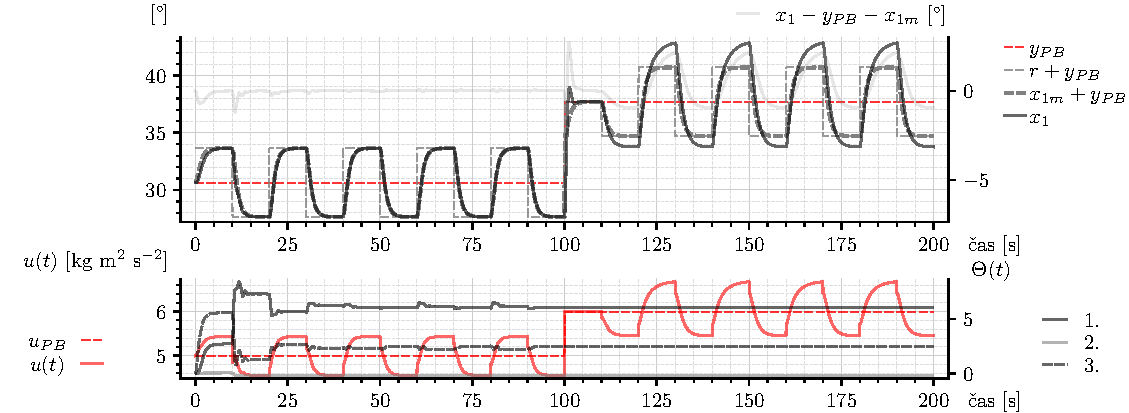
\includegraphics{figsc_ar05_Kyvadlo_ep3_3.pdf}
	}
    \makebox[\textwidth][c]{%
	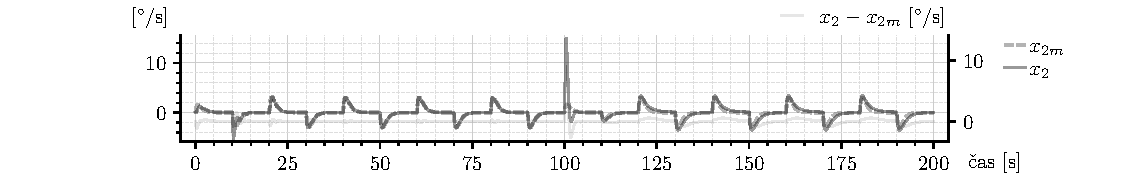
\includegraphics{figsc_ar05_Kyvadlo_ep3_x2_3.pdf}
	}

    \vspace{-2mm}

	\caption{}
	\label{figsc_ar05_Kyvadlo_ep3_3}

    \vspace{-2mm}

\end{figure}



Je zrejmé, že ak bol riadiaci systém naadaptovaný v jednom pracovnom bode, v~inom už nespĺňa cieľ radenia.


% \vfill

Zapnime preto adaptáciu aj po prechode do nového pracovného bodu. Výsledok je na obr.~\ref{figsc_ar05_Kyvadlo_ep3_4}. Parametre riadiaceho systému sa adaptovali na nový pracovný bod.





\begin{figure}[!t]
	\centering

    \vspace{-3mm}

	\makebox[\textwidth][c]{%
	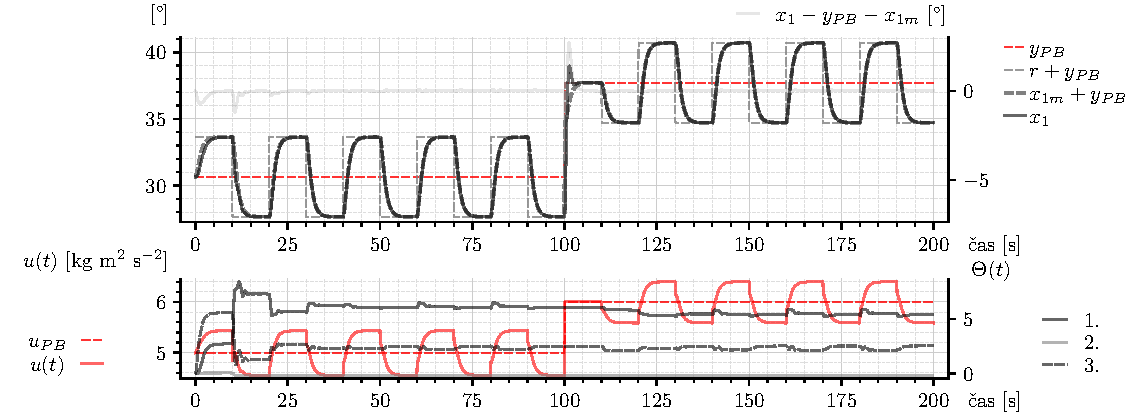
\includegraphics{figsc_ar05_Kyvadlo_ep3_4.pdf}
	}
    \makebox[\textwidth][c]{%
	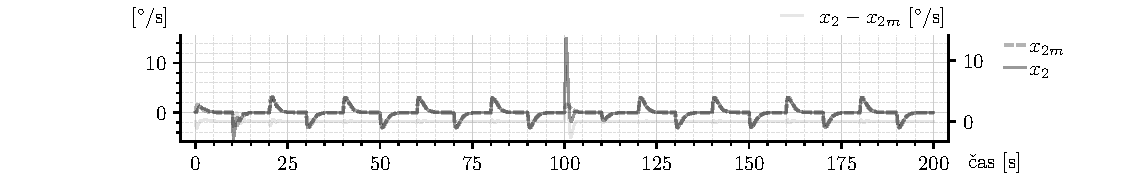
\includegraphics{figsc_ar05_Kyvadlo_ep3_x2_4.pdf}
	}

    \vspace{-2mm}

	\caption{}
	\label{figsc_ar05_Kyvadlo_ep3_4}

    \vspace{-2mm}

\end{figure}





Môžme spraviť aj zmenu na iný pracovný bod, napríklad na  $u_{PB} = 9$. Výsledok je na obr.~\ref{figsc_ar05_Kyvadlo_ep3_5}.



\vfill

\phantom{}
















\section{Otázky a úlohy}
% \addcontentsline{toc}{section}{Otázky a úlohy}







\begin{enumerate}[leftmargin=0pt, labelsep=4mm, itemsep=0pt]


    \item Parametre riadeného systému sú: $\displaystyle A = \begin{bmatrix} 0 & 1 \\ -2 & 1 \end{bmatrix}$, $\displaystyle b = \begin{bmatrix} 0  \\  1 \end{bmatrix}$. Parametre referenčného modelu sú: $\displaystyle A_m = \begin{bmatrix} 0 & 1 \\ -2 & -3 \end{bmatrix}$, $\displaystyle b_m = \begin{bmatrix} 0  \\  1 \end{bmatrix}$. Vypočítajte parametre ($k$~a~$l$) stavového zákona riadenia $u = k^\mathsf{T}\, x + l\,r$, ktoré zabezpečia, že $x$~sleduje~$x_m$.


    \bigskip




    \item Model riadeného systému je zadaný v tvare prenosovej funkcie:
    		\begin{equation*}
    			\frac{y(s)}{u(s)} = \frac{b_0}{s}
    		\end{equation*}
    	kde $y$ je výstup, $u$ je vstup, $b_0 > 0$ je neznámy parameter systému. Cieľom riadenia je aby výstup $y$ sledoval výstup referenčného modelu $y_m$, ktorý je daný prenosovou funkciou
    	\begin{equation*}
    			\frac{y_m(s)}{r(s)} = \frac{b_m}{s + a_m}
    		\end{equation*}
    		kde $r$ je referenčný signál, $a_m = b_m > 0$ sú známe konštanty. Uvažujte použitie zákona riadenia v tvare
    		\begin{equation*}
    			u = \Theta (r - y)
    		\end{equation*}
    		kde $\Theta$ je parameter zákona riadenia, ktorý je potrebné adaptovať.

    		Navrhnite zákon adaptácie použitím Lyapunovovej teórie stability.









            \begin{figure}[!t]
                \centering
            
                \vspace{-3mm}
            
                \makebox[\textwidth][c]{%
                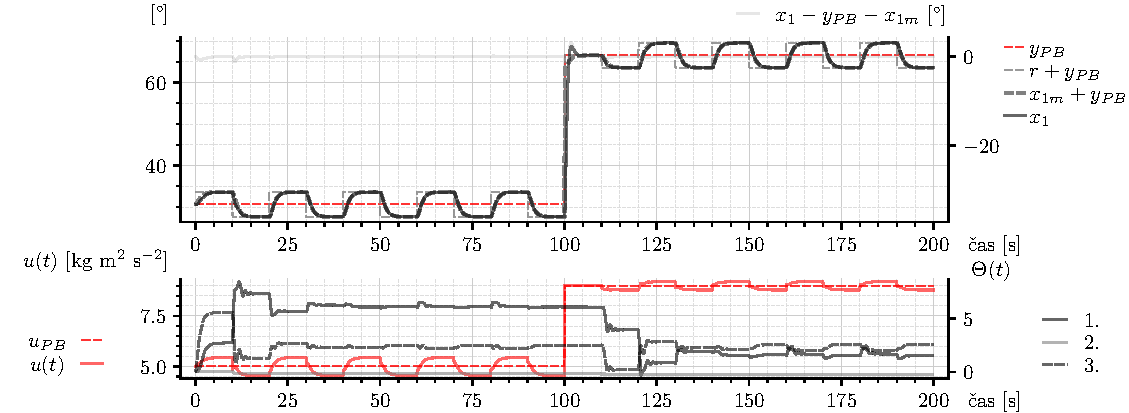
\includegraphics{figsc_ar05_Kyvadlo_ep3_5.pdf}
                }
                \makebox[\textwidth][c]{%
                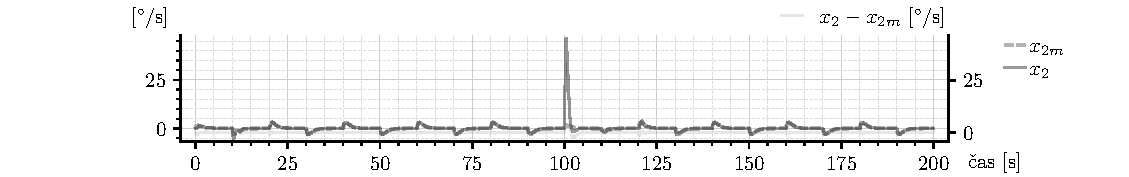
\includegraphics{figsc_ar05_Kyvadlo_ep3_x2_5.pdf}
                }
            
                \vspace{-2mm}
            
                \caption{}
                \label{figsc_ar05_Kyvadlo_ep3_5}
            
                \vspace{-2mm}
            
            \end{figure}
            
            






		\item Je daný model systému
		\begin{align*}
			\dot{x}_1(t) &= x_2(t) \\
			\dot{x}_2(t) &= -a_1 x_2(t) - a_0 x_1(t) + b_0 u(t) \\
			y(t) & = x_1(t)
		\end{align*}
		kde $a_0, a_1, b_0 > 0$ sú neznáme parametre systému, $u(t)$ je vstup, $y(t)$ je výstup a~$x_1(t)$, $x_2(t)$ sú stavové veličiny systému. Tiež je daný referenčný model v tvare
		\begin{align*}
			\begin{bmatrix}
				\dot{x}_{1m}(t) \\ \dot{x}_{2m}(t)
			\end{bmatrix}
			&=
			\begin{bmatrix}
				 0 & 1 \\ -a_{0m} & -a_{1m}
			\end{bmatrix}
			\begin{bmatrix}
				 x_{1m}(t)  \\ x_{2m}(t)
			\end{bmatrix}
			+
			\begin{bmatrix}
				 0  \\  b_{0m}
			\end{bmatrix}
			r(t) \\
			y_m(t)
			&=
			\begin{bmatrix}
				 1 & 0
			\end{bmatrix}
			\begin{bmatrix}
				 x_{1m}(t)  \\ x_{2m}(t)
			\end{bmatrix}
		\end{align*}
		kde $a_{0m}, a_{1m}, b_{0m} > 0$ sú známe parametre referenčného modelu, $r(t)$ je referenčný signál, $y_m(t)$ je výstup a~$x_{1m}(t)$, $x_{2m}(t)$ sú stavové veličiny referenčného modelu.


    \begin{enumerate}
    	\item Navrhnite ideálny stavový regulátor pre zadaný systém, ktorý zabezpečí, že stavové veličiny URO sa správajú rovnako ako stavové veličiny referenčného modelu.
    	\item Navrhnite priamy adaptívny stavový regulátor pre zadaný systém, ktorý zabezpečí, že stavové veličiny URO asymptiticky sledujú stavové veličiny referenčného modelu a zároveň celý adaptívny uzavretý riadiaci obvod je stabilný.
    \end{enumerate}






    \item Odvoďte rovnicu dynamiky stavovej adaptačnej odchýlky pre MRAC so stavovou štruktúrou zákona riadenia.


    \item Navrhnite adaptívny riadiaci systém so stavovým zákonom riadenia a~so zákonom adaptácie navrhnutým pomocou Lyapunovovej teórie stability.

    	\begin{tabular}{@{}l l}
    	Model riadeného systému: & $\begin{array}{@{}l} \dot{x} = A\,x+ b\,u\\   y = c^\mathsf{T}x \end{array}$ \vspace{1.5mm}\\
    	Referenčný model: & $\begin{array}{@{}l} \dot{x}_m = A_m\,x_m + b_m\,r\\   y_m = c^\mathsf{T}_m\,x_m \end{array}$ \vspace{2.5mm} \\
    	Zákon riadenia: & $u = k^\mathsf{T} x + l\,r$
    	\end{tabular}



        \item Nakreslite blokovú schému realizácie adaptívneho riadiaceho systému opísaného nasledovne (podľa možností použite základné bloky ako v Simulinku):
        \begin{align*}
            \dot{x} &= b\,u & &b>0 \\
            \dot{x}_m &= -a_m\,x_m + b_m\,r & &a_m = b_m > 0 \\
            u &= \Theta \, \omega & & \omega = r - x \\
            \dot{\Theta} &= - \gamma\,\omega\,e & &\gamma > 0
        \end{align*}




\end{enumerate}



























\end{document}

